%\documentclass[aspectratio=169]{beamer}
\documentclass{beamer}
\usepackage{minted}
\usepackage[style=numeric]{biblatex}
\usepackage{subfig}
\usepackage{changepage}
%\addbibresource{main.bib}
\usepackage{xcolor}
\usepackage{hyperref}
\usetheme{metropolis}

\definecolor{cvutblue}{RGB}{1,44,86}

\newcommand{\reffig}[1]{Fig.~\ref{#1}}
\newcommand{\reflst}[1]{Lst.~\ref{#1}}
\newcommand{\refalg}[1]{Alg.~\ref{#1}}
\newcommand{\refsec}[1]{Sec.~\ref{#1}}
\newcommand{\reftab}[1]{Table~\ref{#1}}
\newcommand{\refeq}[1]{\eqref{#1}}

\newcommand{\todo}[1]{{\color{red} TODO {#1}}}

\setbeamercolor{palette primary}{bg=cvutblue,fg=white}
\setbeamercolor{background canvas}{bg=white}
%\setbeamercolor{title separator}{fg=cvutblue}

\setbeamertemplate{footline}[frame number]

\setbeamersize{text margin left=6mm, text margin right=6mm} 

\setbeamertemplate{itemize item}{%
  \raisebox{.2ex}{\usebeamercolor[fg]{itemize item}\rule{1ex}{1ex}}%
}
\setbeamercolor{itemize item}{fg=cvutblue}

\metroset{block=fill}

\newcounter{questionnumber}
\newcommand{\questionframe}[3]{
    \stepcounter{questionnumber}
    {
    \setbeamertemplate{footline}{}
    \begin{frame}[plain]%{Question \arabic{questionnumber}}
        \addtocounter{framenumber}{-1}
        \begin{block}{#1}
        \vspace{0.1cm}
            #2
        \end{block}
            #3
    \setbeamertemplate{footline}[frame number]
    \end{frame}
    }
}


\title{Relative Pose Estimation Using Event-Based Measurements of LED Signals}
\subtitle{Thesis Defense}

\date{10.6.2025}
\author{Jakub Pelc}

\institute{Faculty of Electrical Engineering, Czech Technical University in Prague \\ Multi-robot Systems Group}
\begin{document}
\maketitle

\begin{frame}{Assignment}

\small{
\begin{enumerate}
    \item Research the working principles of event-based cameras. Research the existing Visible Light Positioning (VLP) methods such as Received Signal Strength Ratio (RSSR).
    \item Analyze the response of a static event-based camera to UV LEDs used by the UVDAR localization system in UAV swarms. Modulate the signals with varying frequency, relative distance, and angle.
    \item Design an approach for relative pose estimation of UAV swarm members, utilizing the analysis results and a proper
fisheye lens calibration method.
    \item Implement the proposed solution for a Robot Operating System (ROS). Test the implementation on the data used for
the response analysis and discuss the results.
    \item Conduct a real-world UAV swarming experiment. Compare the estimation results with a GNSS ground truth. 
\end{enumerate}
}

\end{frame}

% ------------- EVENT CAMERAS -------------

\begin{frame}{Event-based cameras}

\begin{columns}[T]

\begin{column}{0.48\textwidth}
\vspace{0.3cm}
\begin{itemize}
    \item The event-cameras function by asynchronously generating events (positive or negative), based on pixel-level illumination changes.
    \item They offer a higher dynamic range than traditional cameras but generally require a different approach to data processing.
\end{itemize}

\end{column}

\begin{column}{0.48\textwidth}

    \begin{figure}[H]
        \centering
        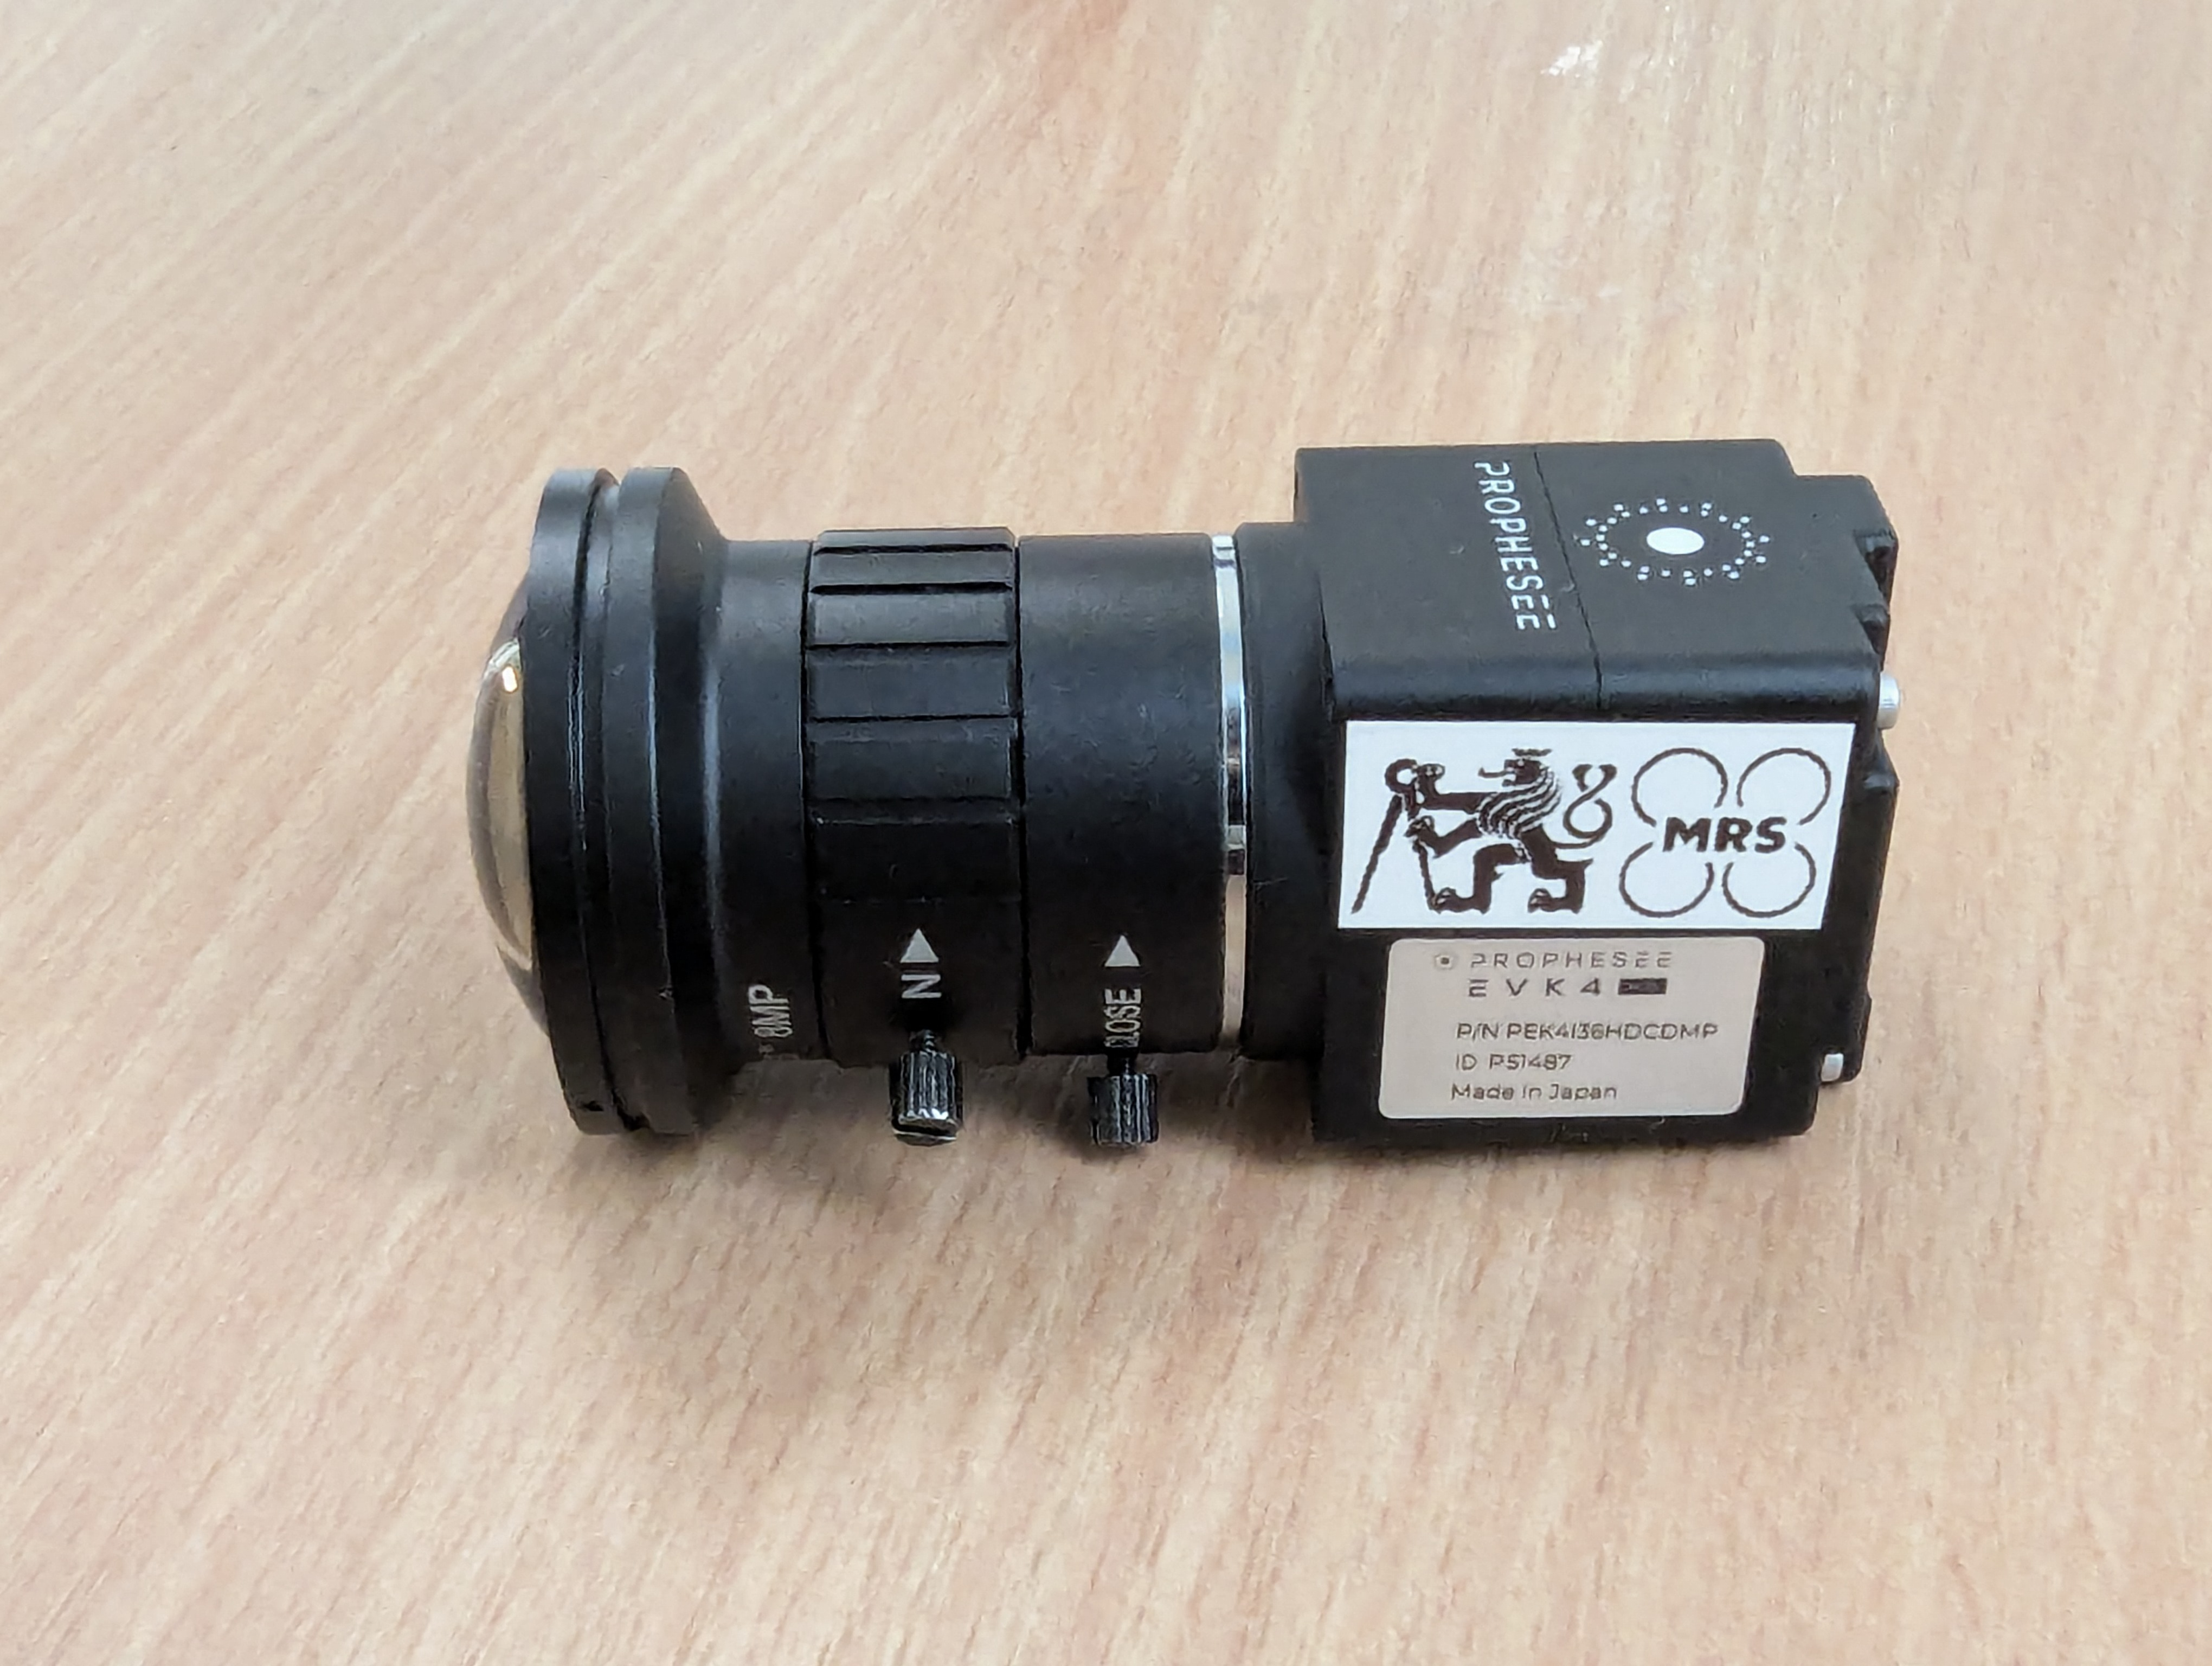
\includegraphics[width=0.85\textwidth]{../fig/photos/evk4.jpg}
        \label{fig:eventcameras1}
    \end{figure}

    \begin{figure}[H]
        \centering
        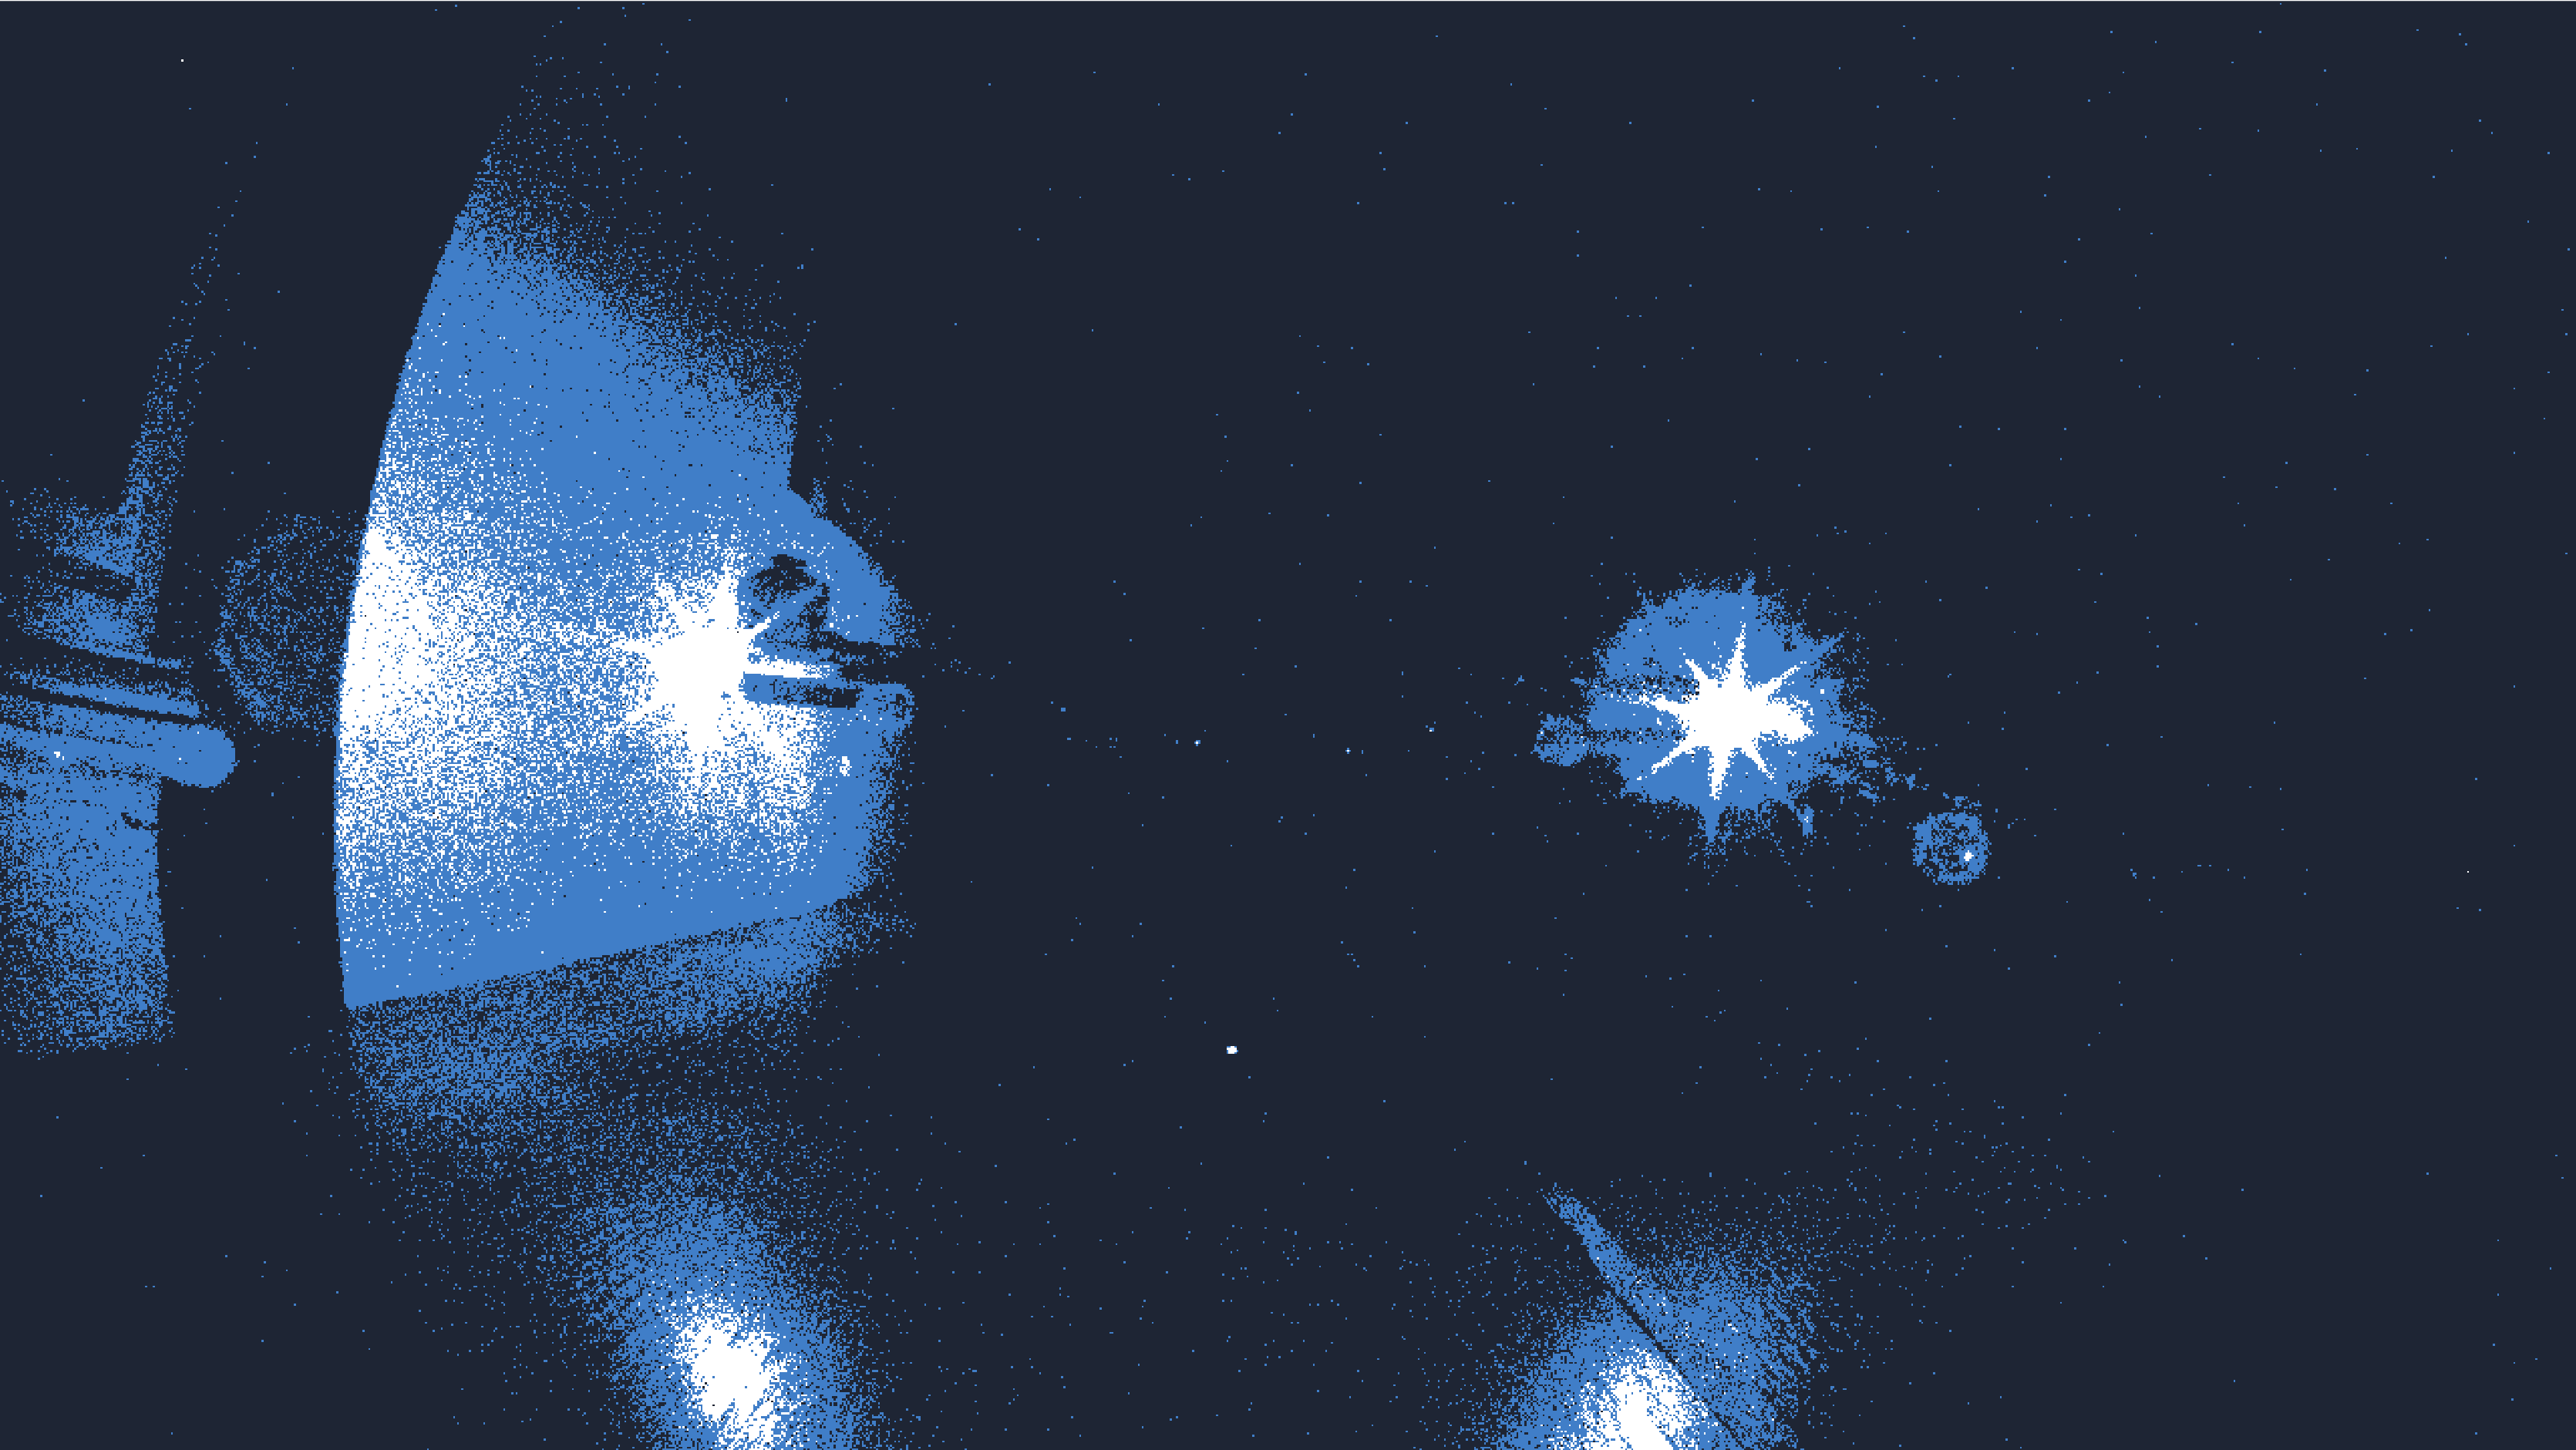
\includegraphics[width=0.85\textwidth]{../fig/photos/meas1.png}
        \label{fig:eventcameras2}
    \end{figure}

\end{column}

\end{columns}

\end{frame}
% ---------------- UVDAR ------------------


\begin{frame}{UVDAR}

\begin{columns}[T]

\begin{column}{0.48\textwidth}
    \vspace{0.5cm}
    \begin{itemize}
        \item We use a UAV equipped with the UVDAR system, which controls the UV LEDs and allows their modulation.
        \item The camera is equipped with a narrowband UV filter to help with the light filtering.
    \end{itemize}
\end{column}

\begin{column}{0.48\textwidth}
    \begin{figure}[H]
        \centering
        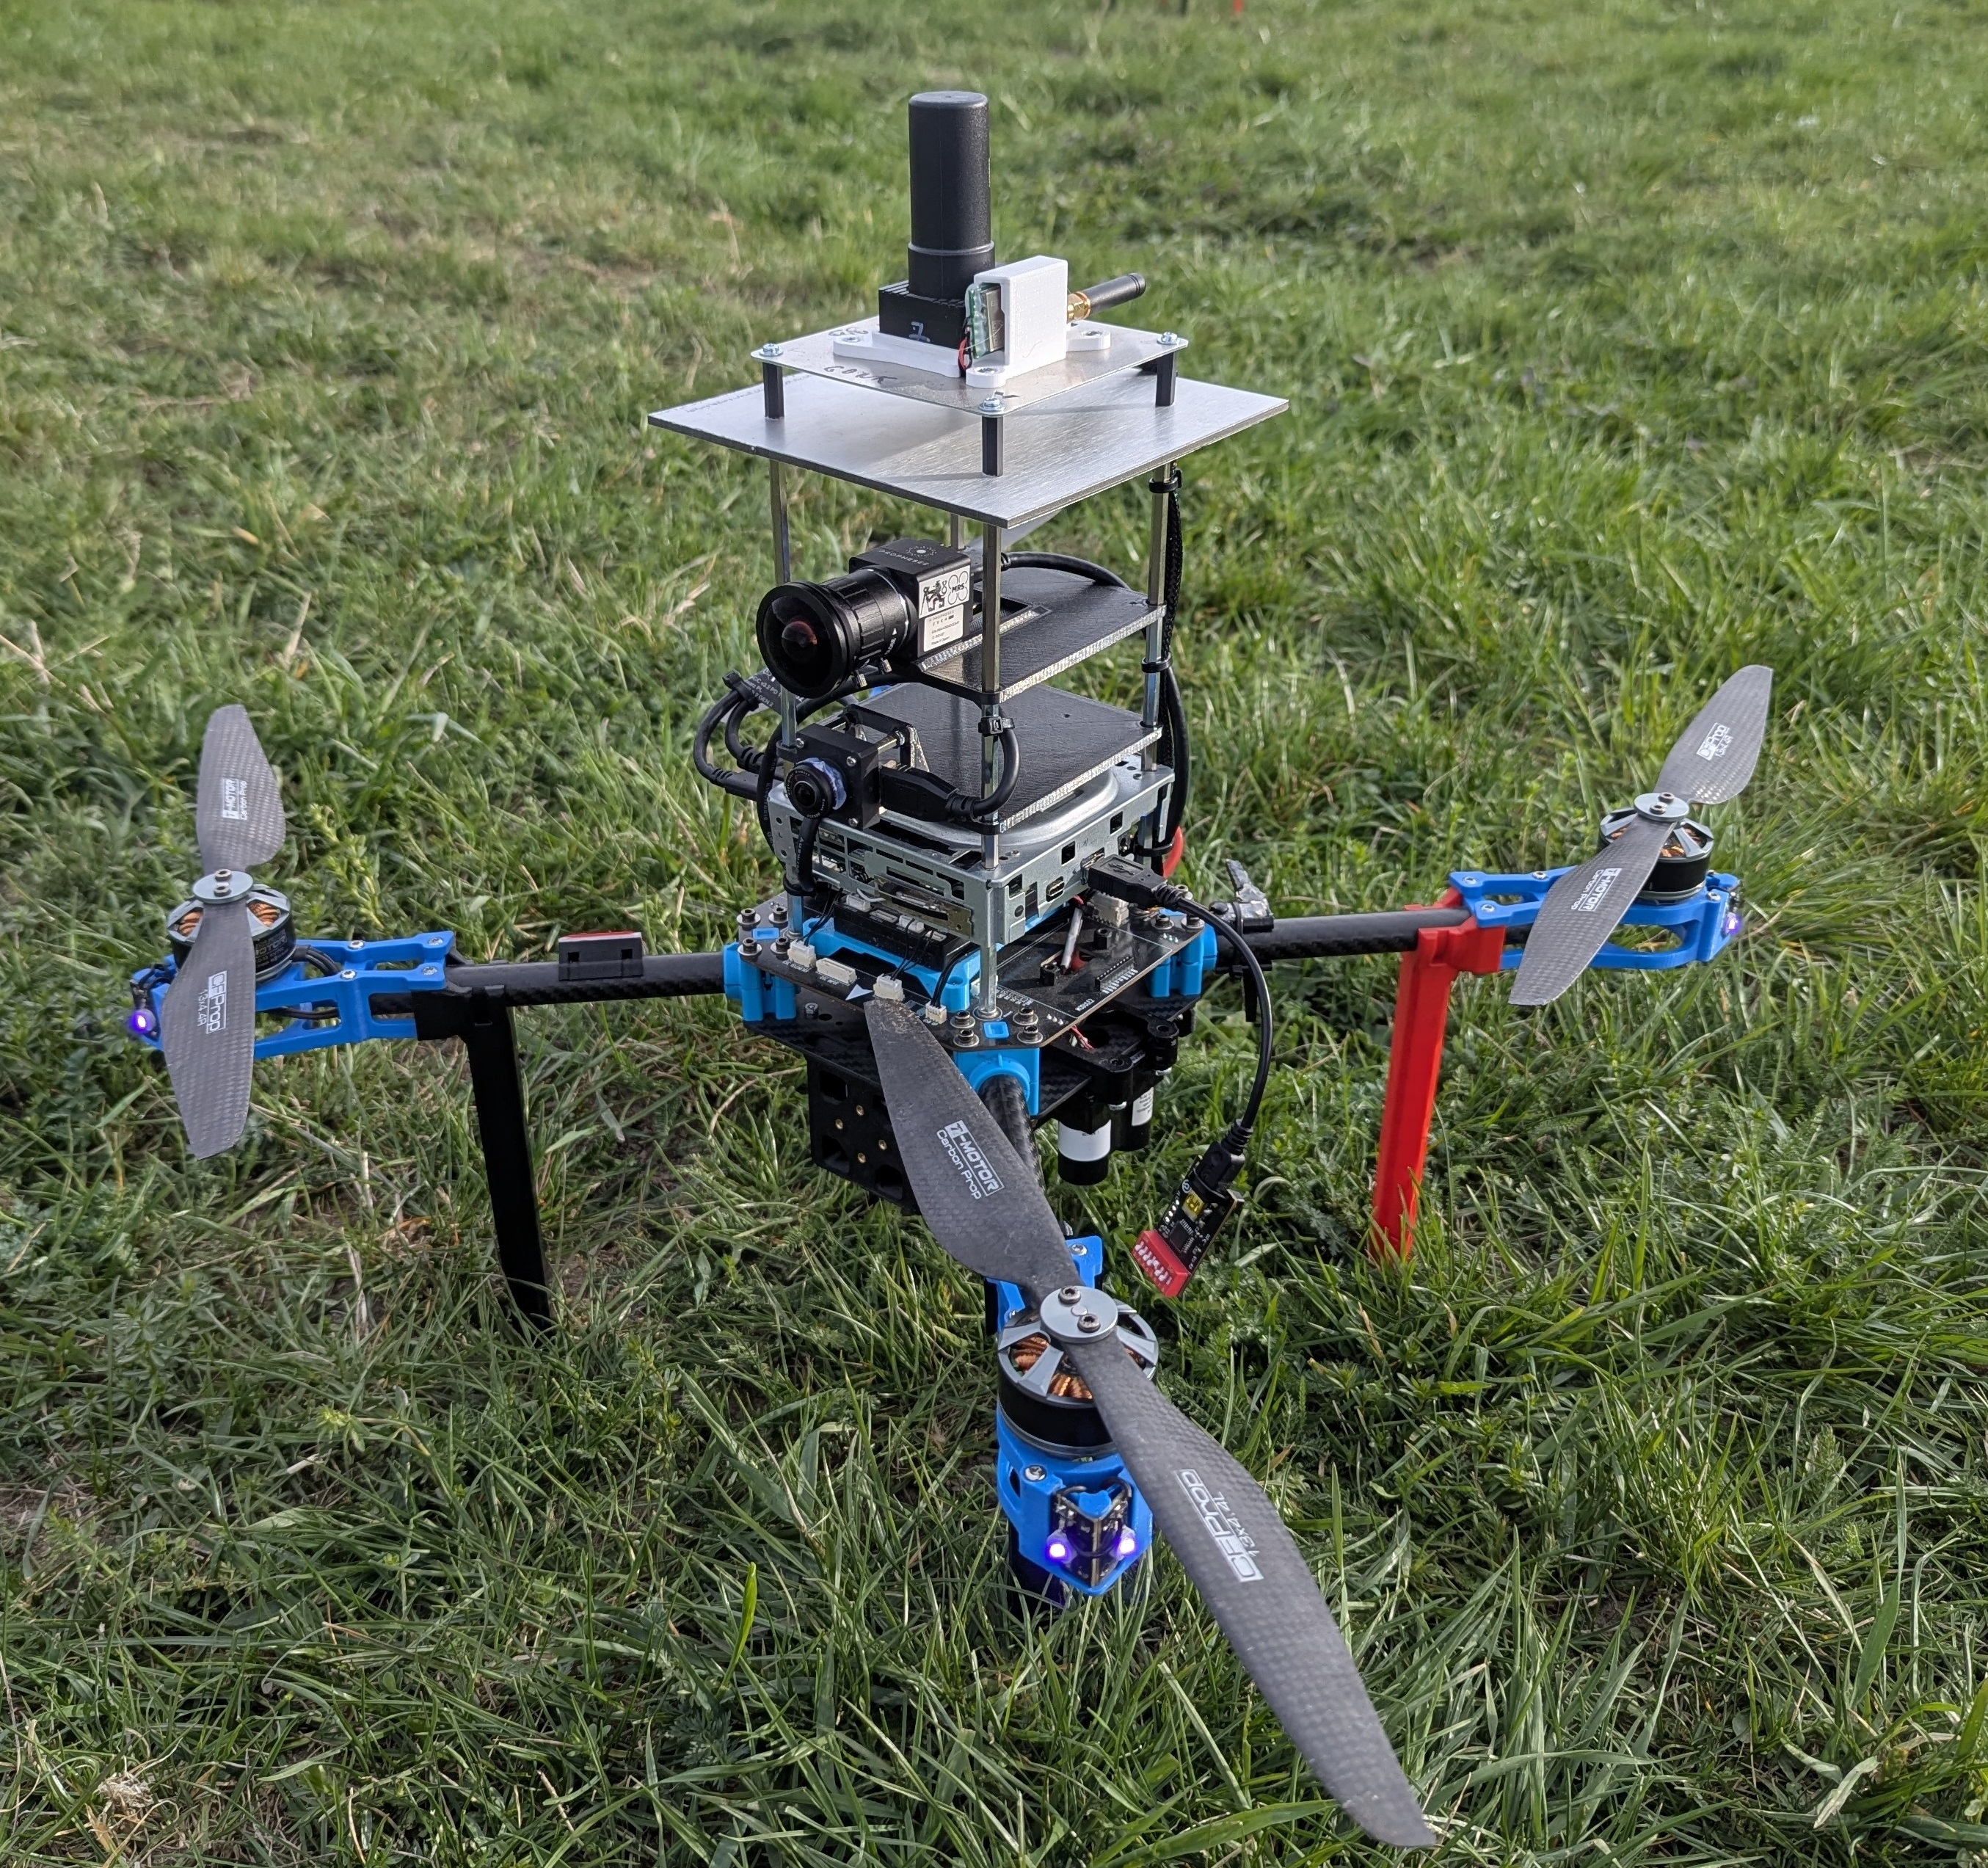
\includegraphics[width=0.99\textwidth]{../fig/photos/uvdar.jpg}
        \label{fig:uvdar}
    \end{figure}
\end{column}

\end{columns}

\end{frame}

% ------------- Event-based camera influence -------------

\begin{frame}{Influence Factors}

\begin{columns}[T]
    % Left column for distance and frequency plots
    \begin{column}{0.48\textwidth}
        \vspace{-0.5cm}
        \begin{figure}[H]
            \centering
            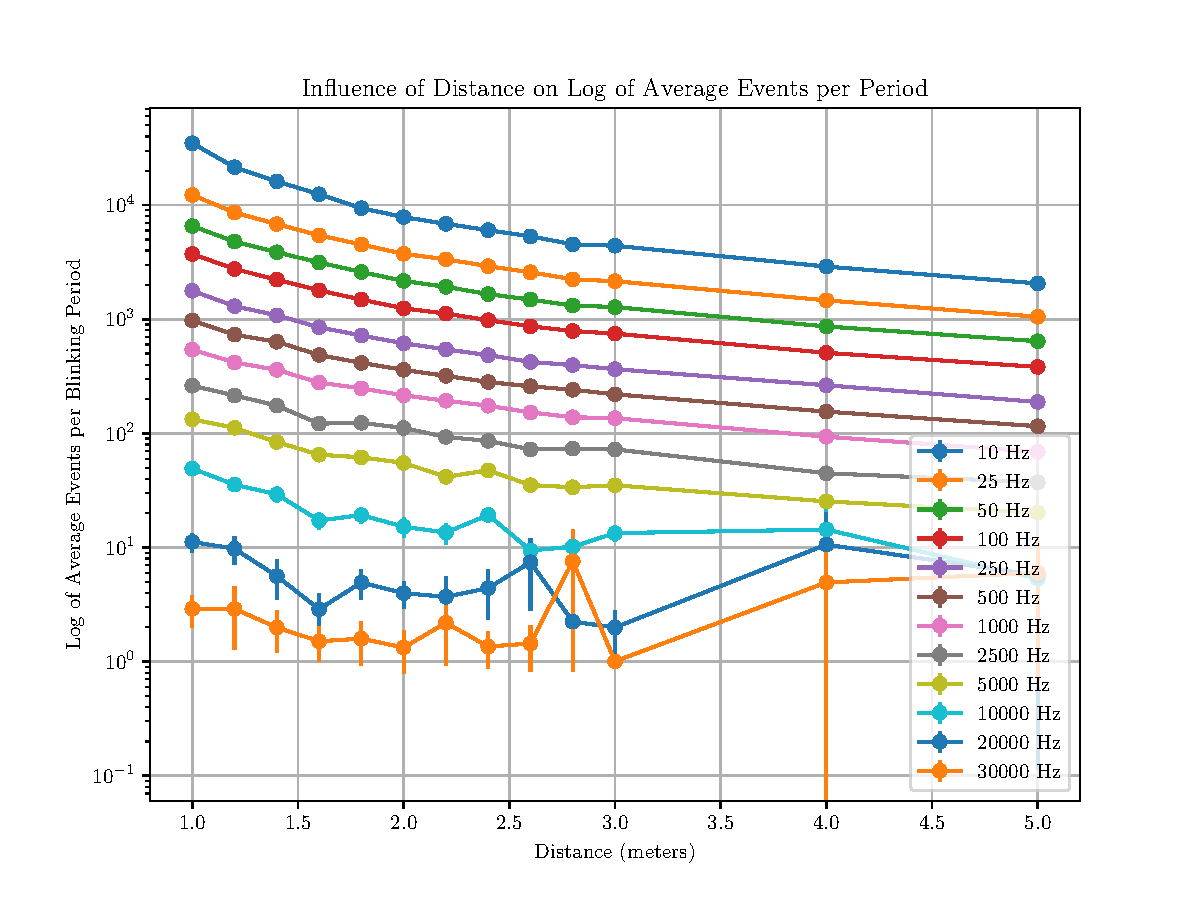
\includegraphics[width=\textwidth]{../fig/semestral/distlog.pdf}
            \label{fig:dist_influence}
            %\caption{Distance influence}
        \end{figure}
        
        \vspace{-1.5cm}
        
        \begin{figure}[H]
            \centering
            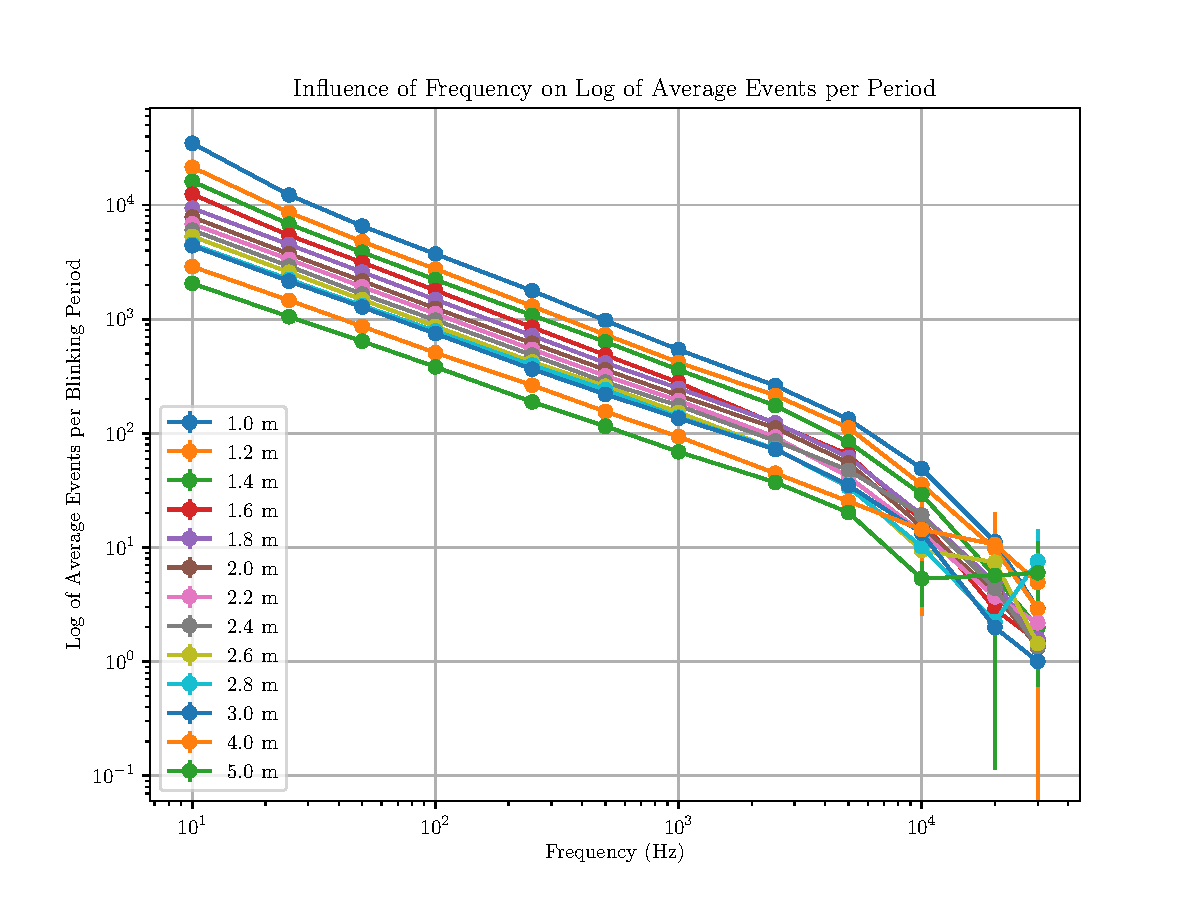
\includegraphics[width=\textwidth]{../fig/semestral/freqlog.pdf}
            \label{fig:freq_influence}
            %\caption{Frequency influence}
        \end{figure}
    \end{column}
    
    \begin{column}{0.48\textwidth}
        \vspace{-0.3cm}
        \begin{figure}[H]
            \centering
            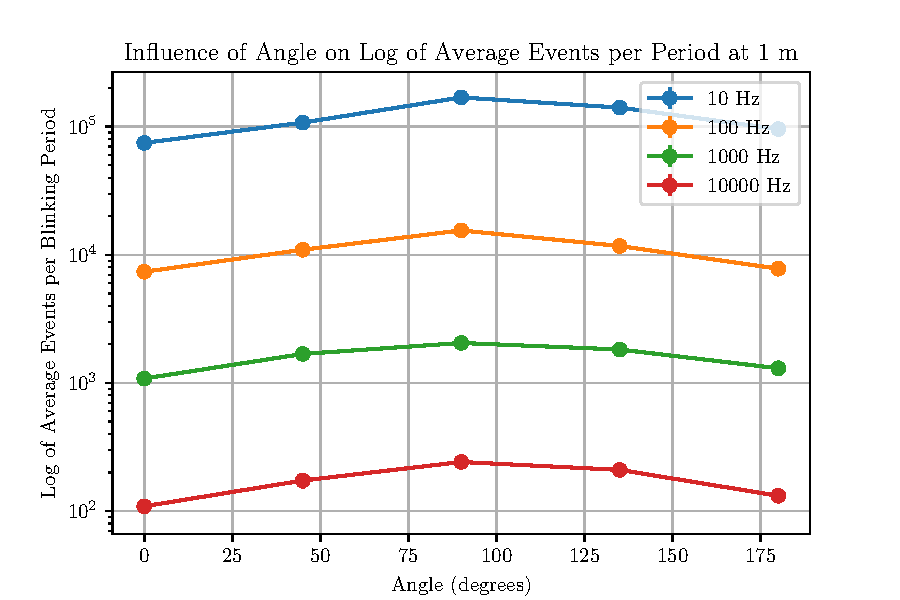
\includegraphics[width=\textwidth]{../fig/semestral/angle2.pdf}
            \label{fig:rotation_influence}
            \caption{Distance, frequency and rotation angle influence}
        \end{figure}
        
        \tiny{
            This is an experimental validation of the
            \begin{itemize}
                \item Inverse square law: $\text{intensity} \propto \frac{1}{\text{distance}^2}$
                \item Emission characteristics of the LEDs used: $I(\theta) = I_0\cos(\theta)$
            \end{itemize}
        }
    \end{column}
\end{columns}

\end{frame}

% ------------- Inverse square law -------------

\begin{frame}{Experimental validation of the inverse square law}

    \begin{figure}
        \centering
        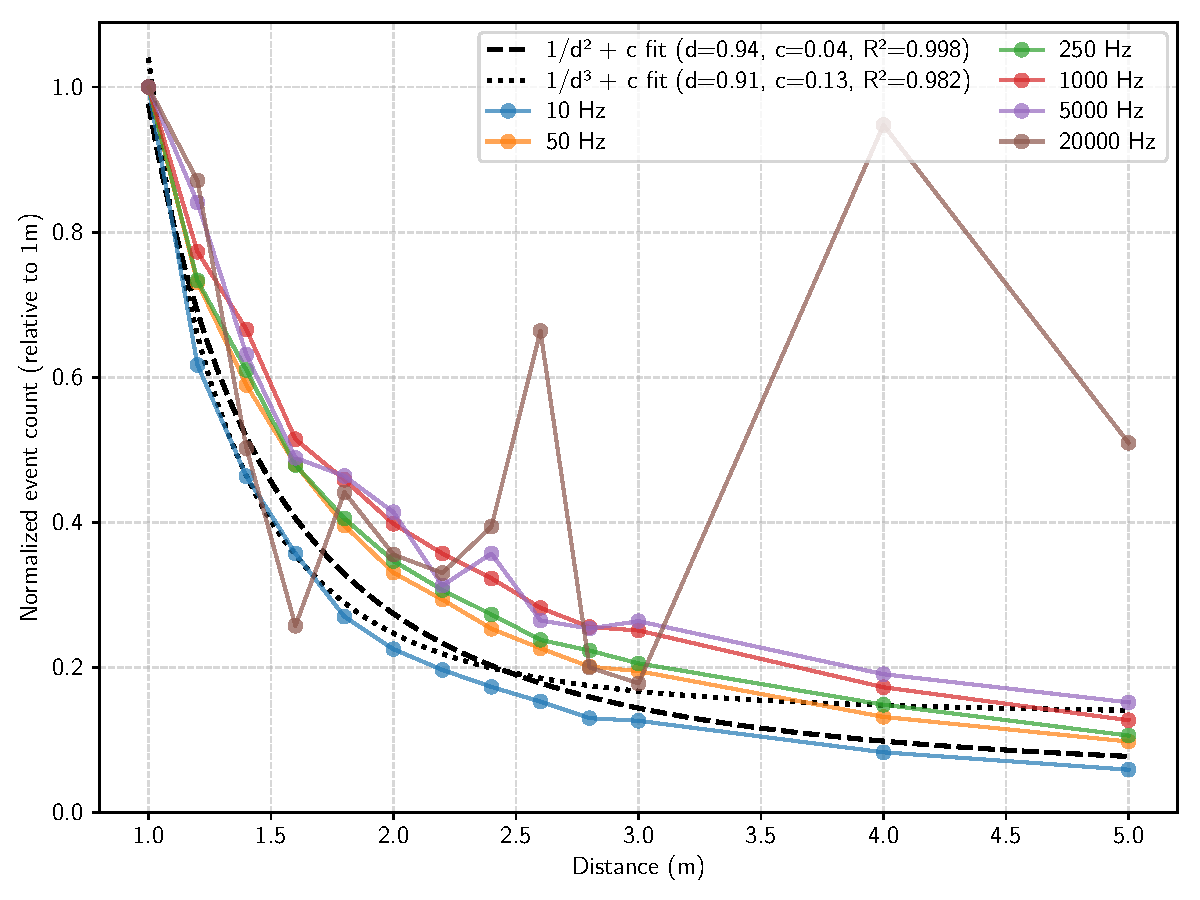
\includegraphics[width=0.70\textwidth]{../fig/pgfplot/build/inv_square.pdf}
        \label{fig:fit1}
        \caption{Experimental validation of the inverse square law: \scriptsize{$\text{intensity} \propto \frac{1}{\text{distance}^2}$}.}
    \end{figure}

    % \vspace{-0.5cm}
    % \begin{equation*}
    %     \text{intensity} \propto \frac{1}{\text{distance}^2}
    % \end{equation*}

\end{frame}

% ------------- Camera calibration -------------

\begin{frame}{Camera calibration}

\begin{columns}[T]
    % Left column for distance and frequency plots
    \begin{column}{0.48\textwidth}
        \vspace{-0.1cm}
        \begin{figure}[H]
            \centering
            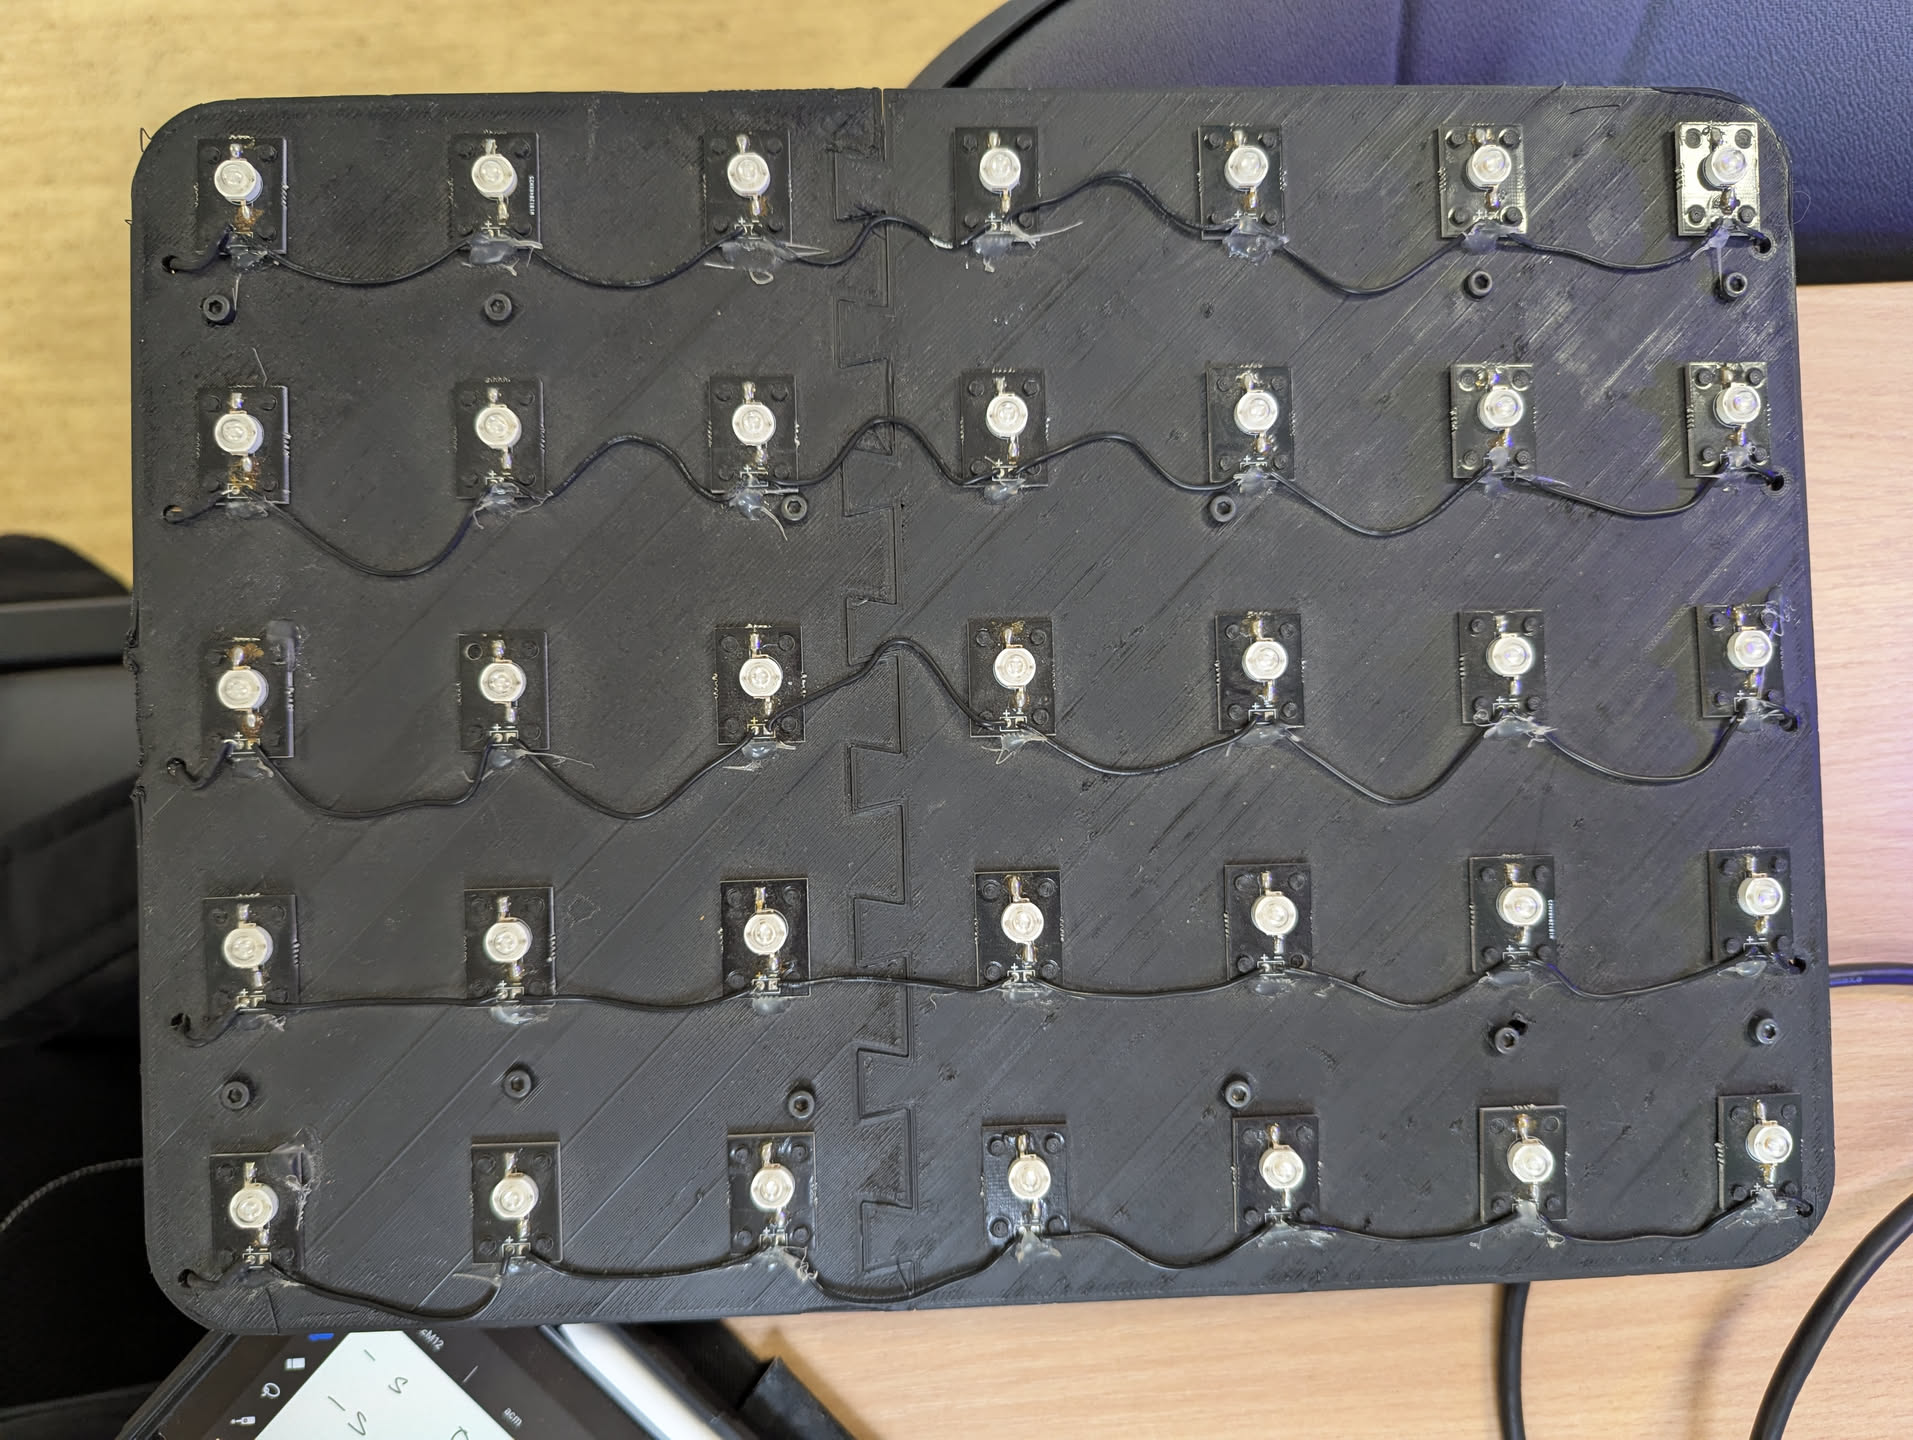
\includegraphics[width=0.8\textwidth]{../fig/photos/lattice.jpeg}
            \label{fig:lattice_img}
            %\caption{Distance influence}
        \end{figure}
        
        \vspace{0.1cm}
        
        \begin{figure}[H]
            \centering
            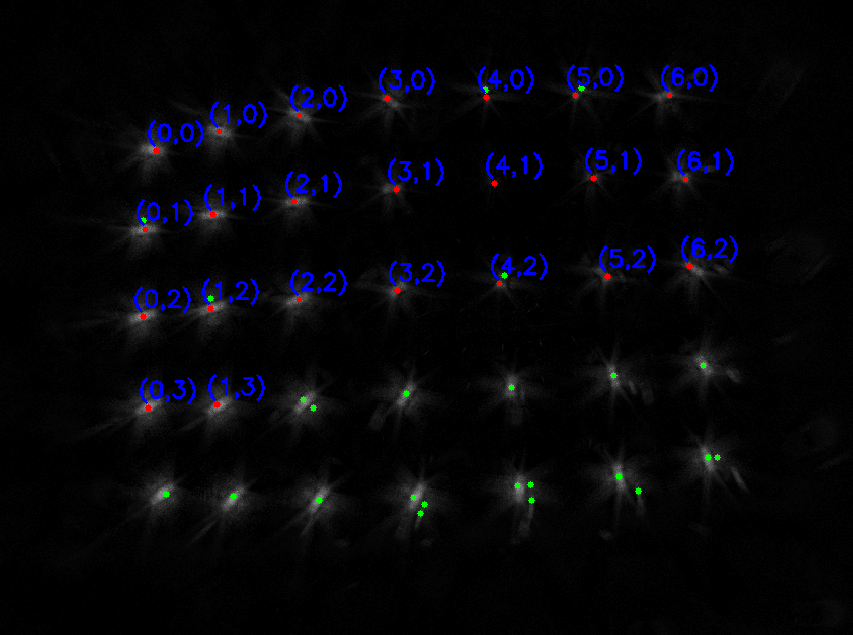
\includegraphics[width=0.8\textwidth]{../fig/photos/lattice_blobs1.png}
            \label{fig:lattice_evs}
            %\caption{Frequency influence}
        \end{figure}
    \end{column}
    
    \begin{column}{0.48\textwidth}
        \vspace{-0.3cm}
        \begin{figure}[H]
            \centering
            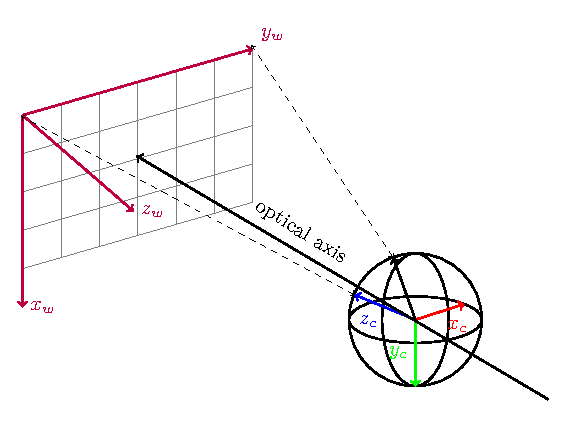
\includegraphics[width=\textwidth]{../fig/tikz/extrinsic.pdf}
            \label{fig:extrinsic_img}
            \caption{Camera calibration grid of $5\times7$ UV LEDs}
        \end{figure}
        
        \tiny{
            The point labeling order needs to be consistent across calibration frames to facilitate correct results.
        }
    \end{column}
\end{columns}
    
\end{frame}

\begin{frame}{Camera calibration results}
\framesubtitle{Ellipse fitting and calibration outcomes}

\begin{columns}[T]
    \begin{column}{0.49\textwidth}
        \vspace{-0.2cm}
        \begin{figure}
            \centering
            %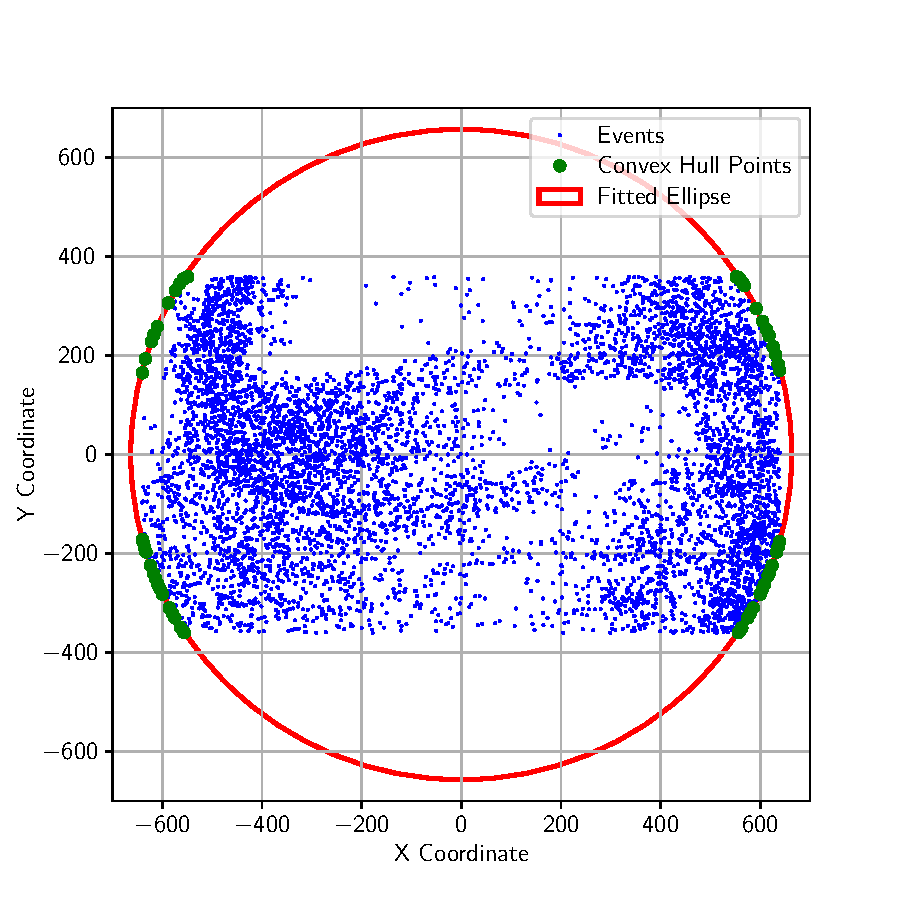
\includegraphics[width=0.70\textwidth]{./fig/pgfplot/build/ellipse_hull.pdf}
            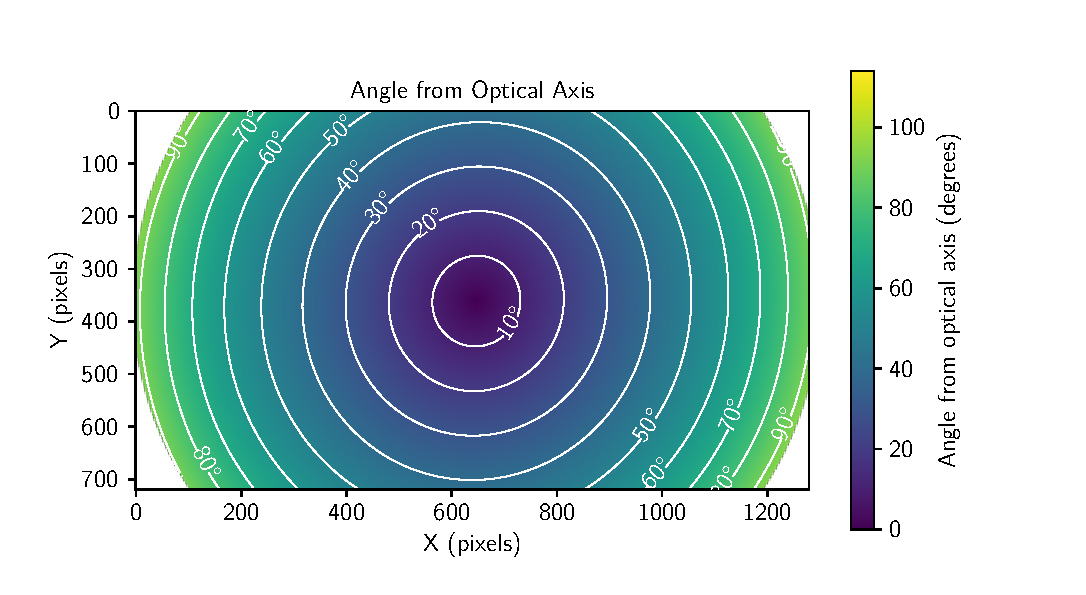
\includegraphics[width=\textwidth]{./fig/pgfplot/build/evk4_viz.pdf}
            
            %\vspace{0.2cm} % Adjust spacing between images
            
            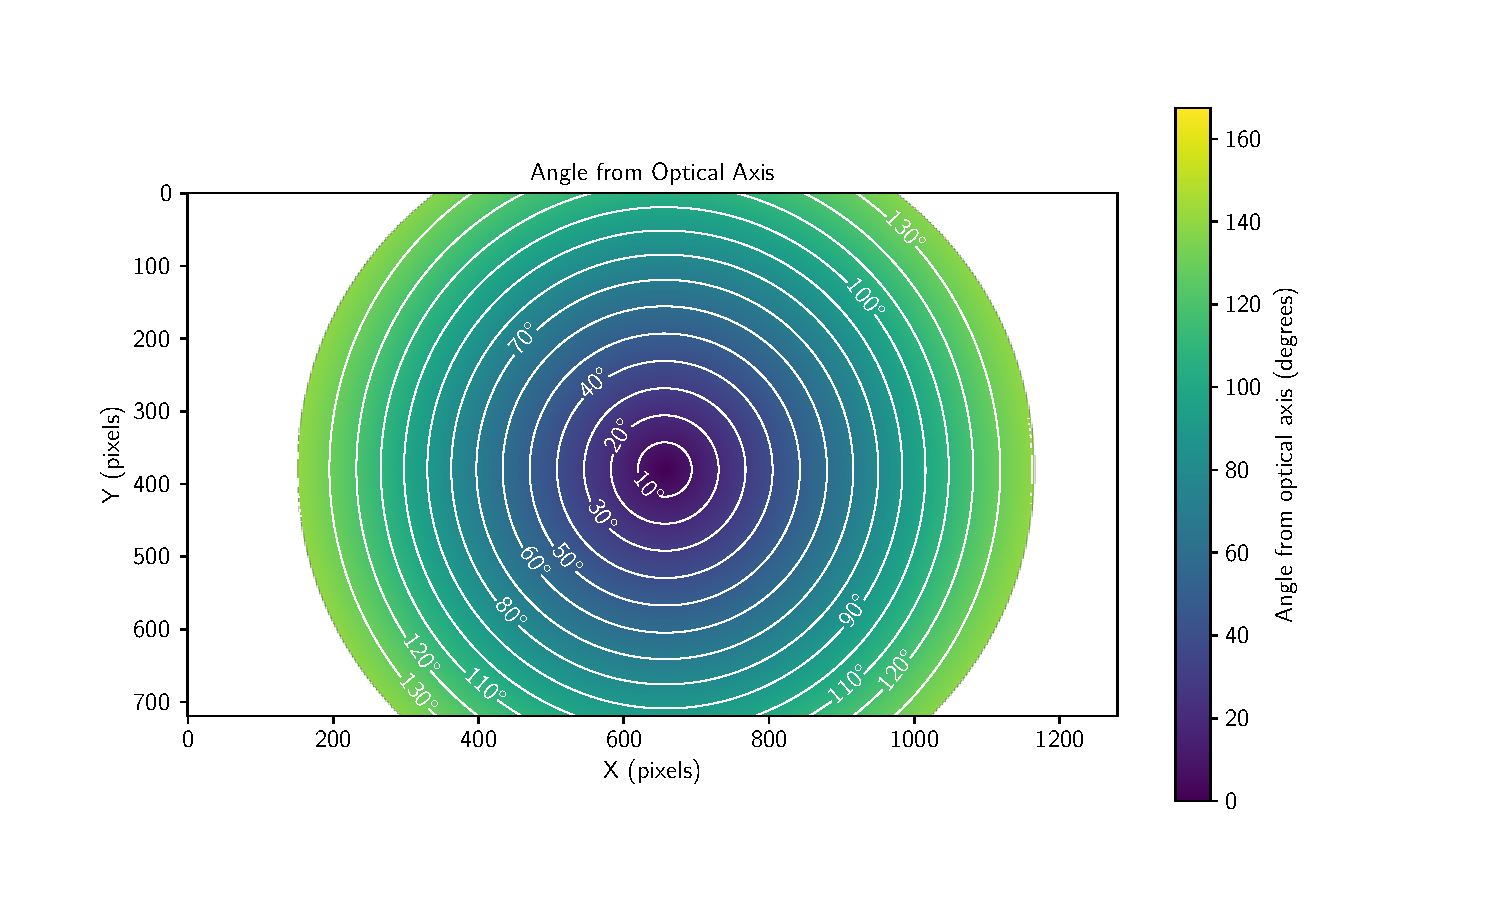
\includegraphics[width=\textwidth]{./fig/pgfplot/build/viz_ent.pdf}
            
            \caption{Lens visible area reconstruction}
            \label{fig:ellipse}
        \end{figure}
    \end{column}
    
    % Right column - Results images
    \begin{column}{0.49\textwidth}
        \vspace{-0.5cm}
        \begin{figure}
            \centering
            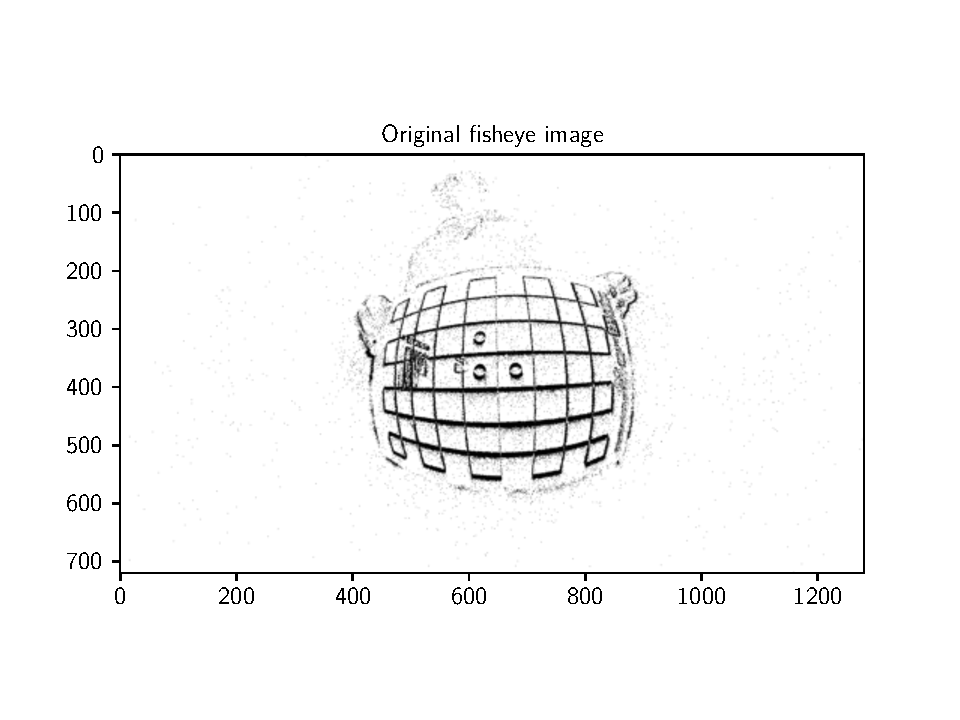
\includegraphics[width=0.88\textwidth]{./fig/pgfplot/build/ent_before.pdf}
            
            \vspace{-0.6cm}
            
            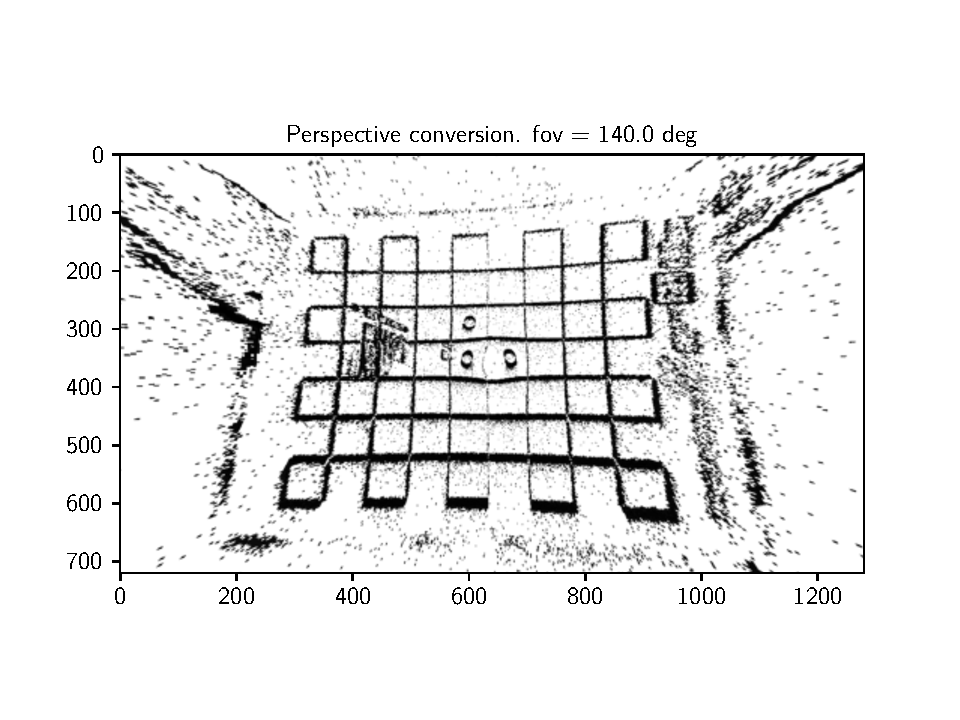
\includegraphics[width=0.88\textwidth]{./fig/pgfplot/build/ent_after.pdf}
            
            \caption{Lens before and after calibration}
            \label{fig:calib_after}
        \end{figure}
    \end{column}
\end{columns}

\end{frame}

% ------------- PnP -------------

\begin{frame}{Perspective-n-Point}

\begin{figure}[H]
    \centering
    \raisebox{0.2\height}{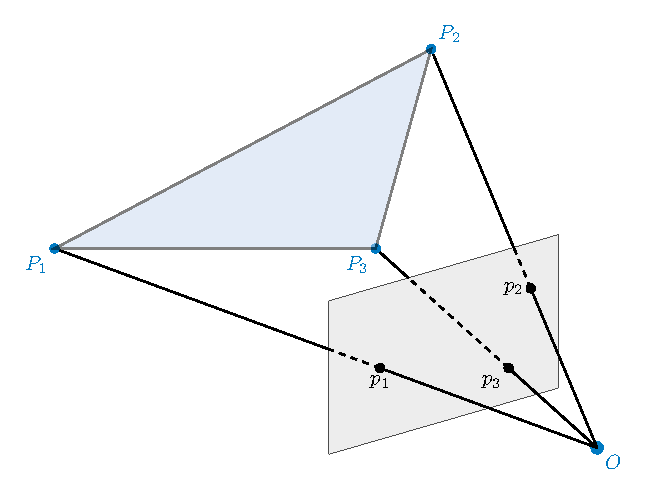
\includegraphics[width=0.55\textwidth]{../fig/tikz/p3p.pdf}}%
    \hspace{1em}%
    \raisebox{0.5\height}{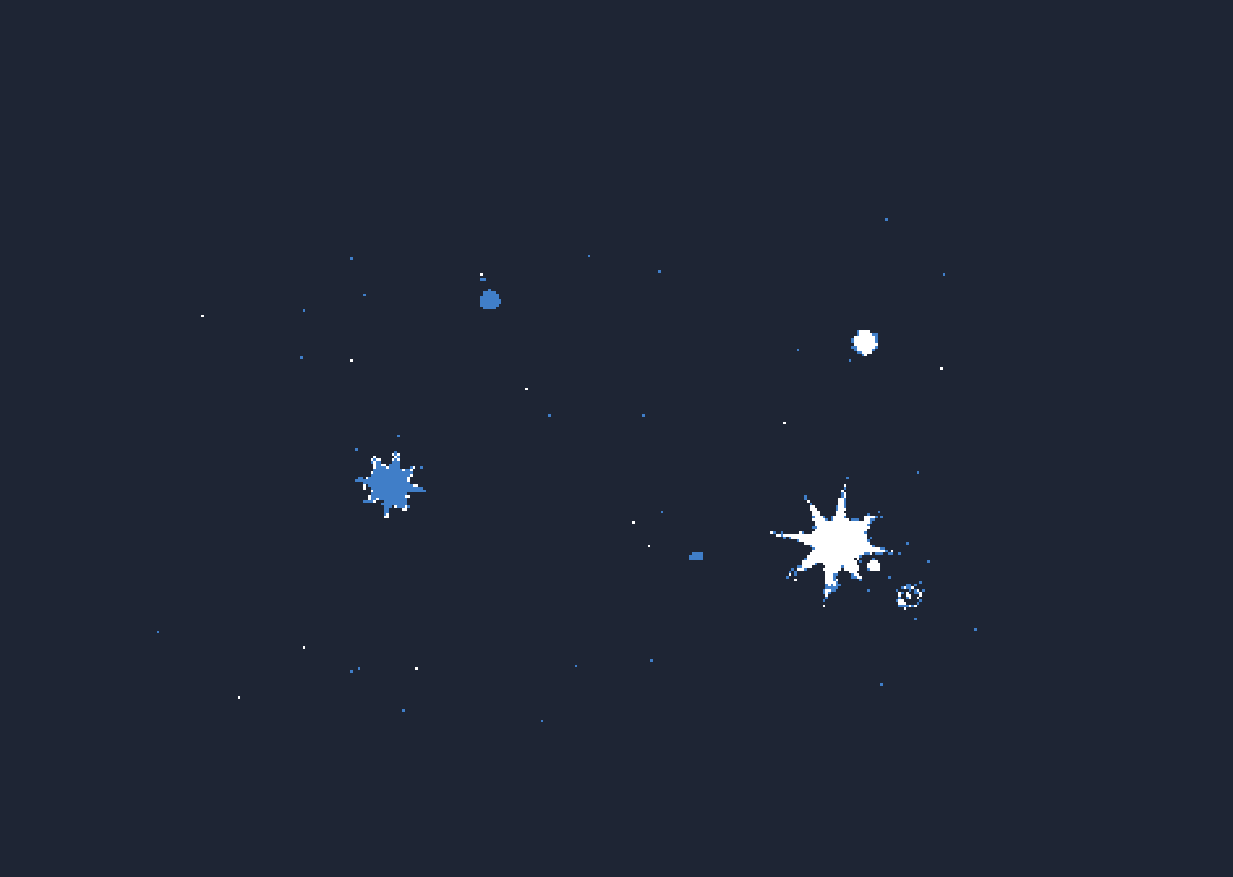
\includegraphics[width=0.40\textwidth]{../fig/photos/pnpmeas.png}}
    \label{fig:pnp}
    \caption{Perspective-n-Point visualisation.}
\end{figure}

A minimum of 3 points is required for a pose estimation using PnP.

\end{frame}

% ------------- ROS -------------

\begin{frame}{ROS implementation}

    \begin{figure}
        \centering
        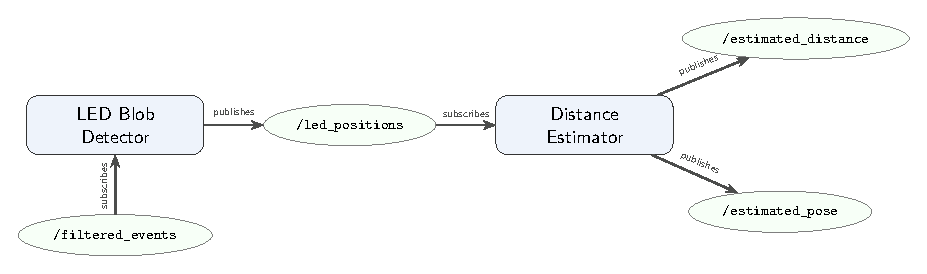
\includegraphics[width=1.0\textwidth]{../fig/tikz/rosflow.pdf}
        \label{fig:ros}
        \caption{ROS position and distance estimation pipeline.}
    \end{figure}

\end{frame}

% ------------- Experiments, results -------------

\begin{frame}{Experiments}

\begin{figure}[H]
	\centering
	\subfloat[Static experiment] {
	  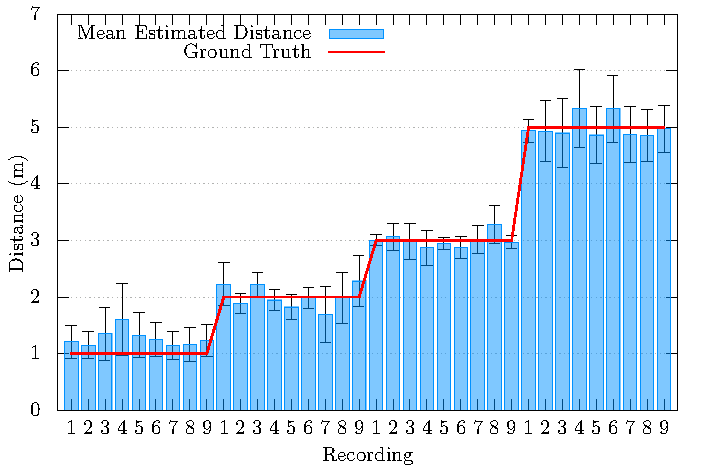
\includegraphics[width=0.45\textwidth]{../fig/tikz/pnp_results.pdf}
	  \label{fig:static_experiment}
	}
	\subfloat[Flying experiment] {
	  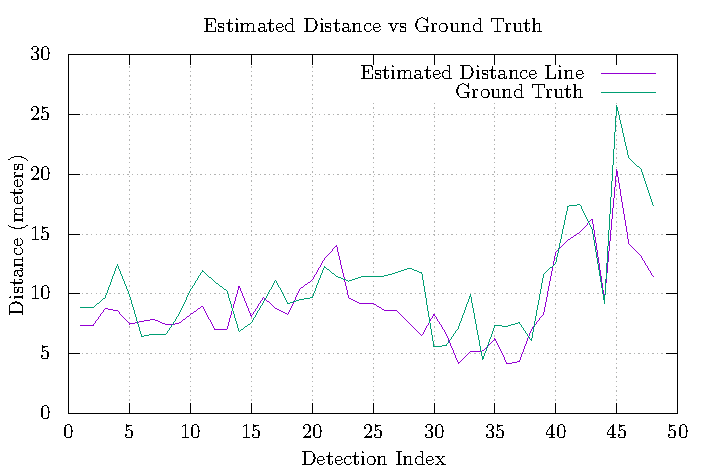
\includegraphics[width=0.49\textwidth]{../fig/tikz/experiment_analysis.pdf}
	  \label{fig:flying_experiment}
	}
	\caption{
            The distance estimation results with a mean error of
            $0.34 \pm 0.16$ meters for the static experiment, and
            $2.47 \pm 1.75$ meters for the flying experiment.
        }
	\label{fig:experiment_results}
\end{figure}

\end{frame}

\begin{frame}{Experiments}

\begin{figure}[H]
	\centering
	  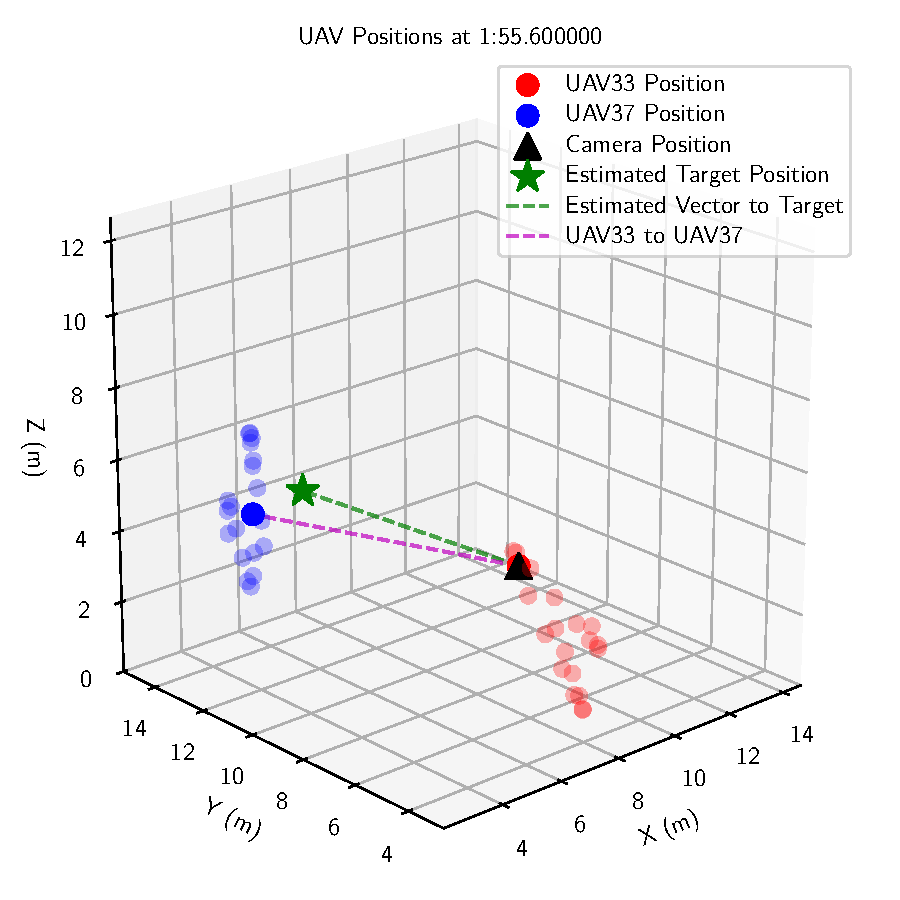
\includegraphics[width=0.45\textwidth]{../fig/pgfplot/build/3dplot2.pdf}
	  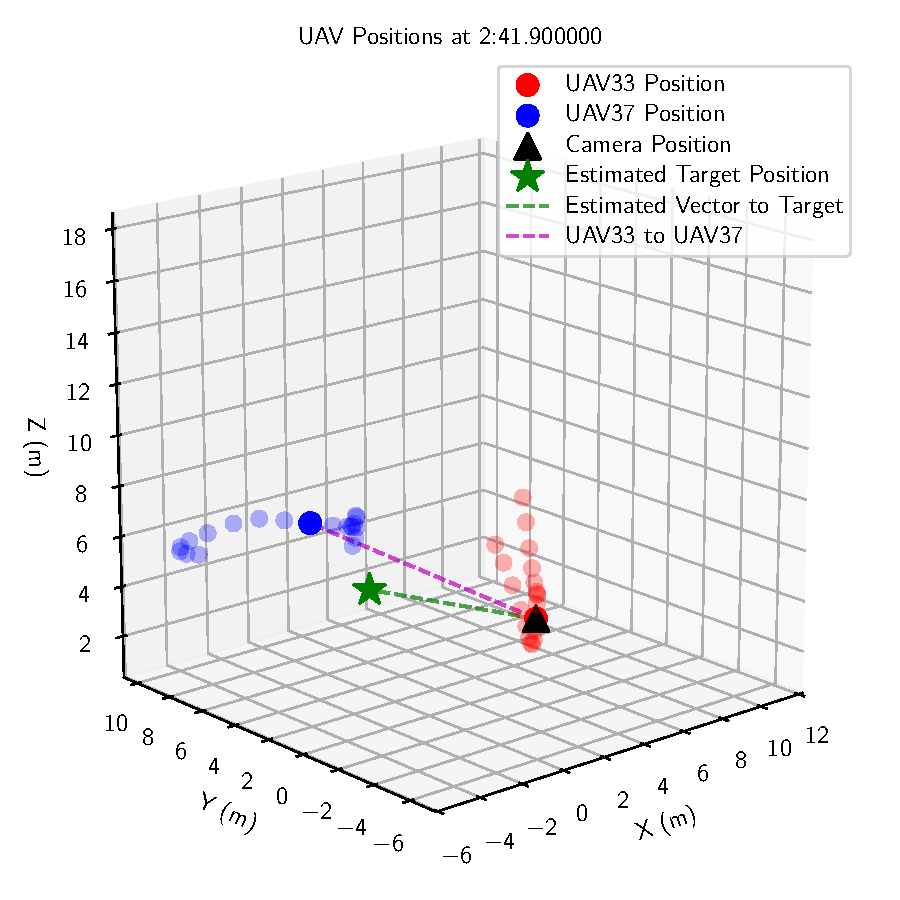
\includegraphics[width=0.45\textwidth]{../fig/pgfplot/build/3dplot1.pdf}
	\caption{
           Pose estimation results, with the estimated pose highlighted in green, and the real pose of the UAVs highlighted in red and blue.
        }
	\label{fig:poseresults}
\end{figure}

\end{frame}

% -------------------- CONCLUSION ---------------------

\begin{frame}{Conclusion}

\begin{columns}[T]
    \begin{column}{0.49\textwidth}
        \vspace{0.5cm}
        \scriptsize{
            \begin{itemize}
                \item The response of the event-based camera to the UV LEDs was measured and analyzed with varying distances, frequencies, and angles.
                \item Calibration of the camera with fisheye lenses was performed.
                \item A ROS node was implemented to facilitate automatic pose and distance estimation from detected LED centers.
                \item A flying experiment was performed with two flying UAVs, each equipped with an event-based camera and a fisheye lens.
                \item The results have shown an estimation accuracy of tens of centimeters in static cases, and in meters range during active motion and large distances.
            \end{itemize}
        }
    \end{column}

    \begin{column}{0.49\textwidth}
        \vspace{-0.1cm}
        \begin{figure}
            \centering
            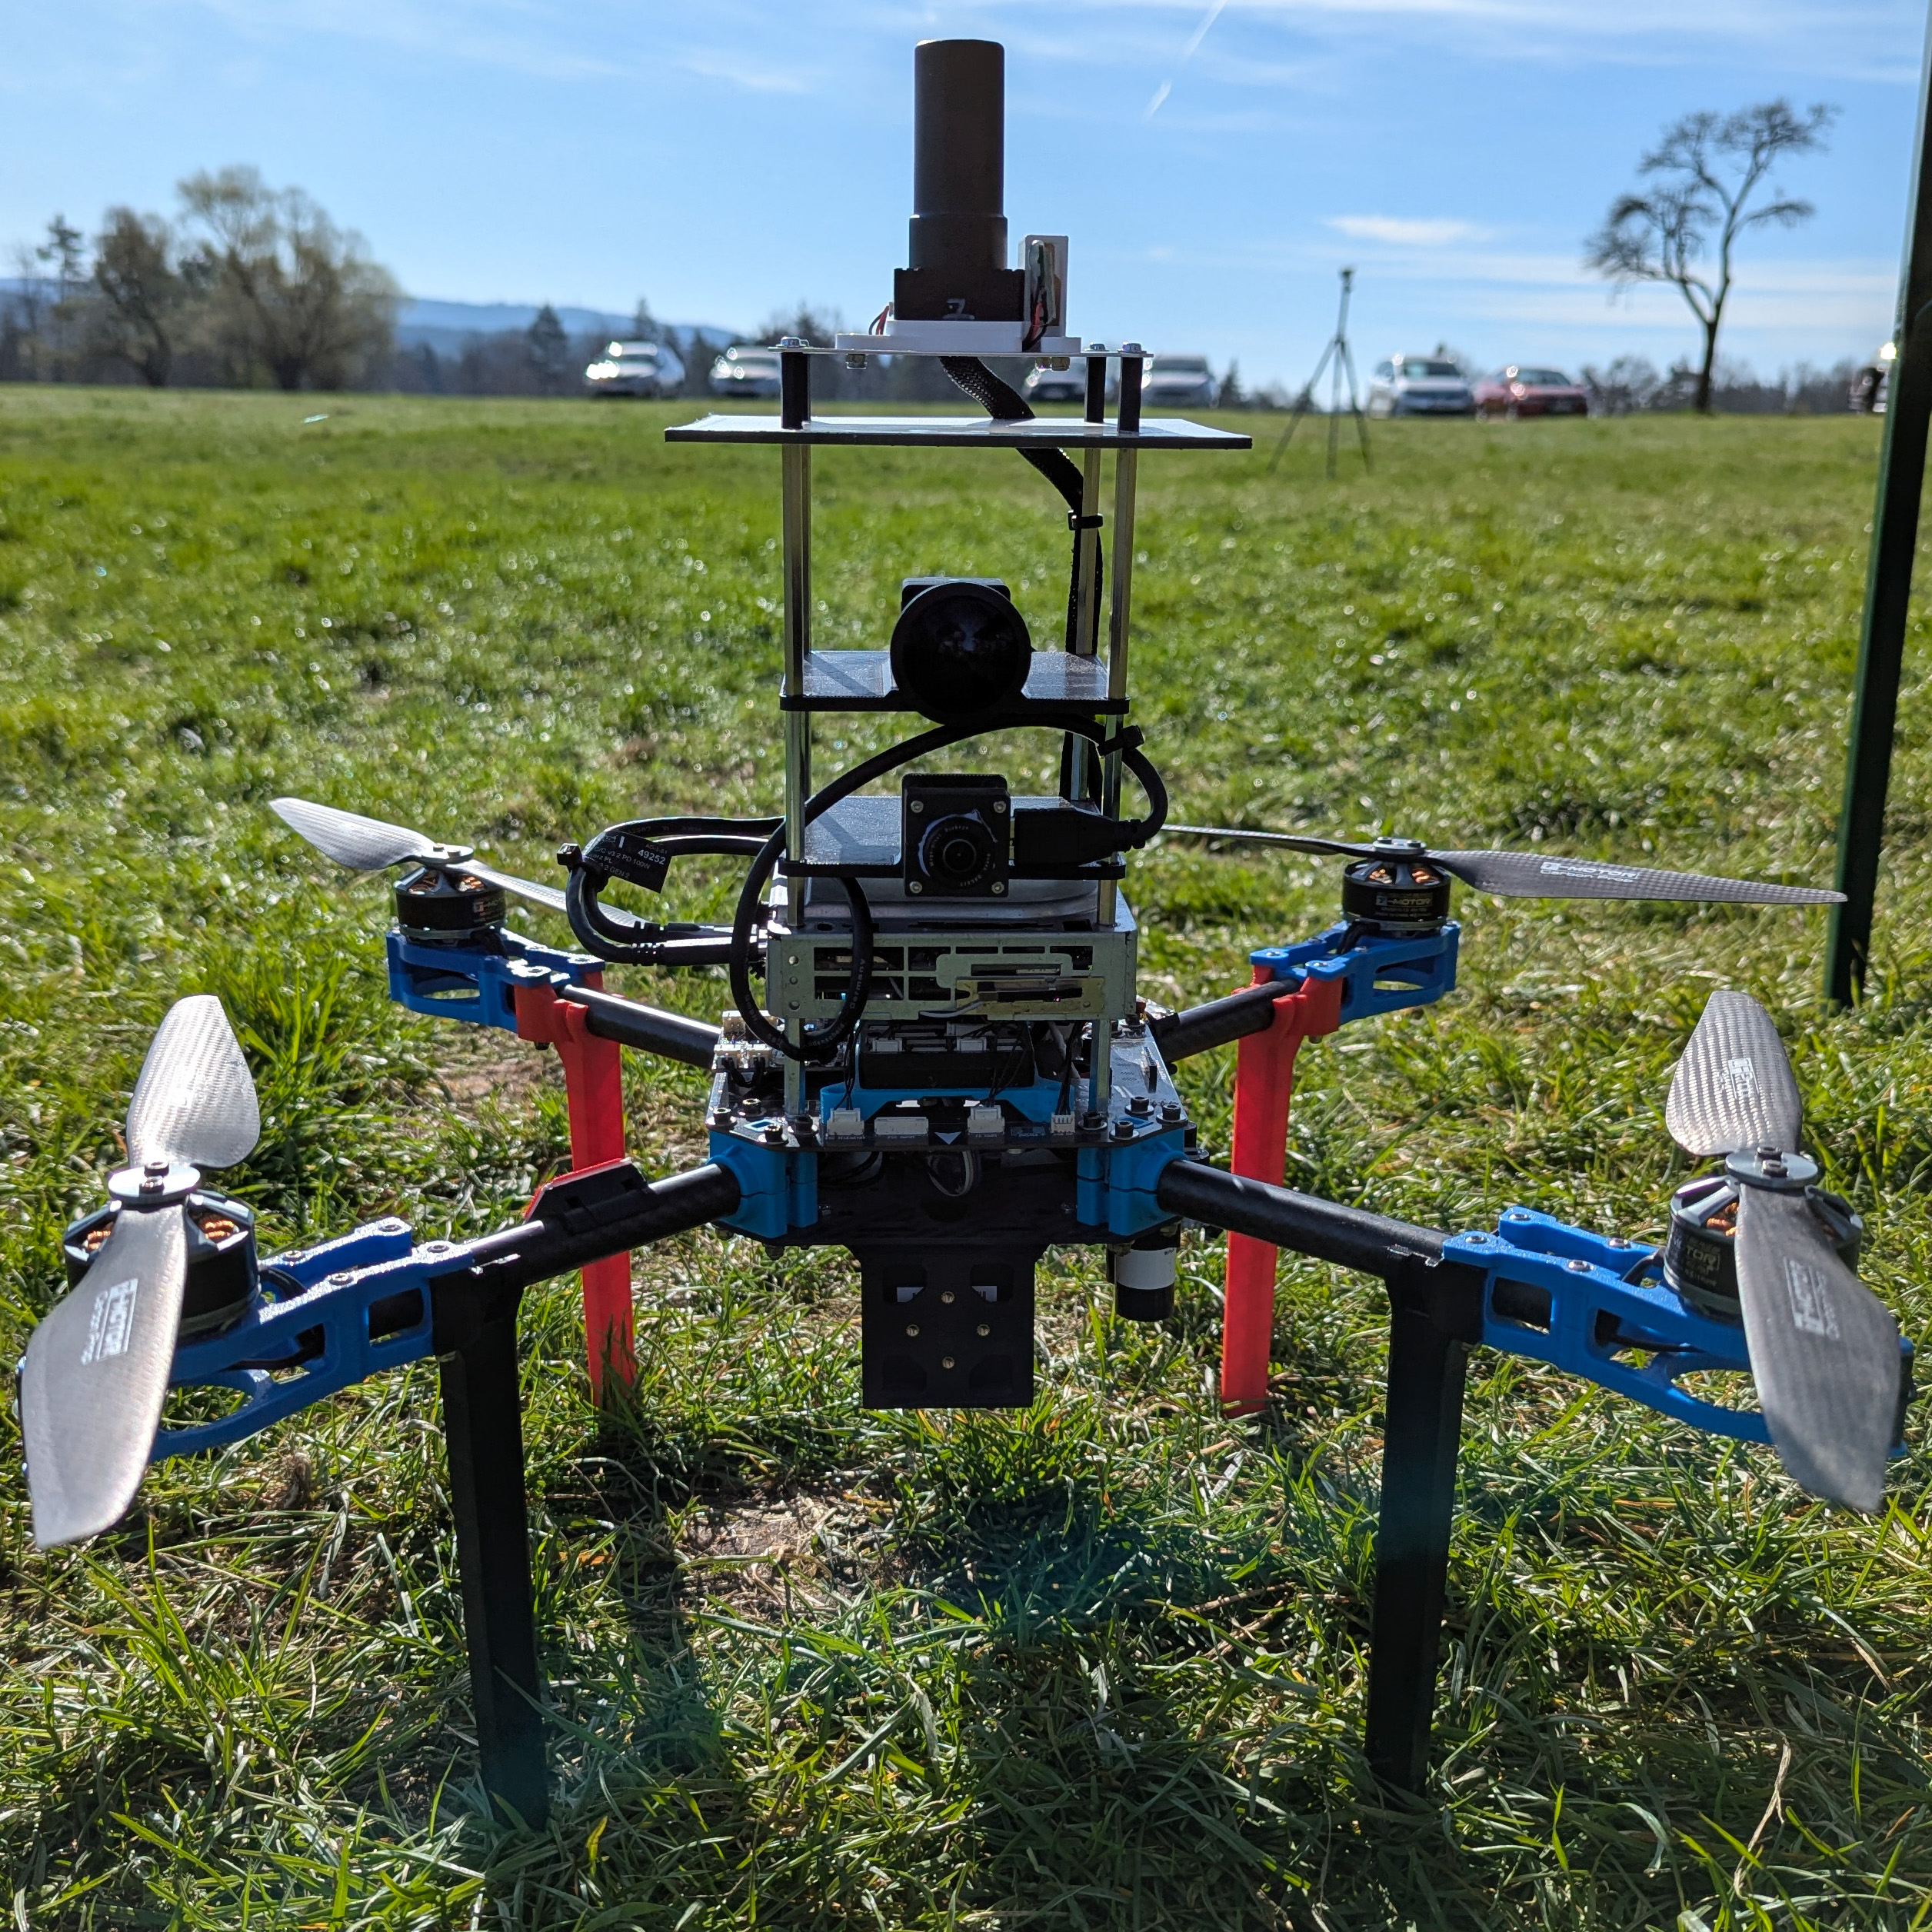
\includegraphics[width=0.60\textwidth]{./fig/photos/uav33.jpg}
            
            \vspace{0.1cm}
            
            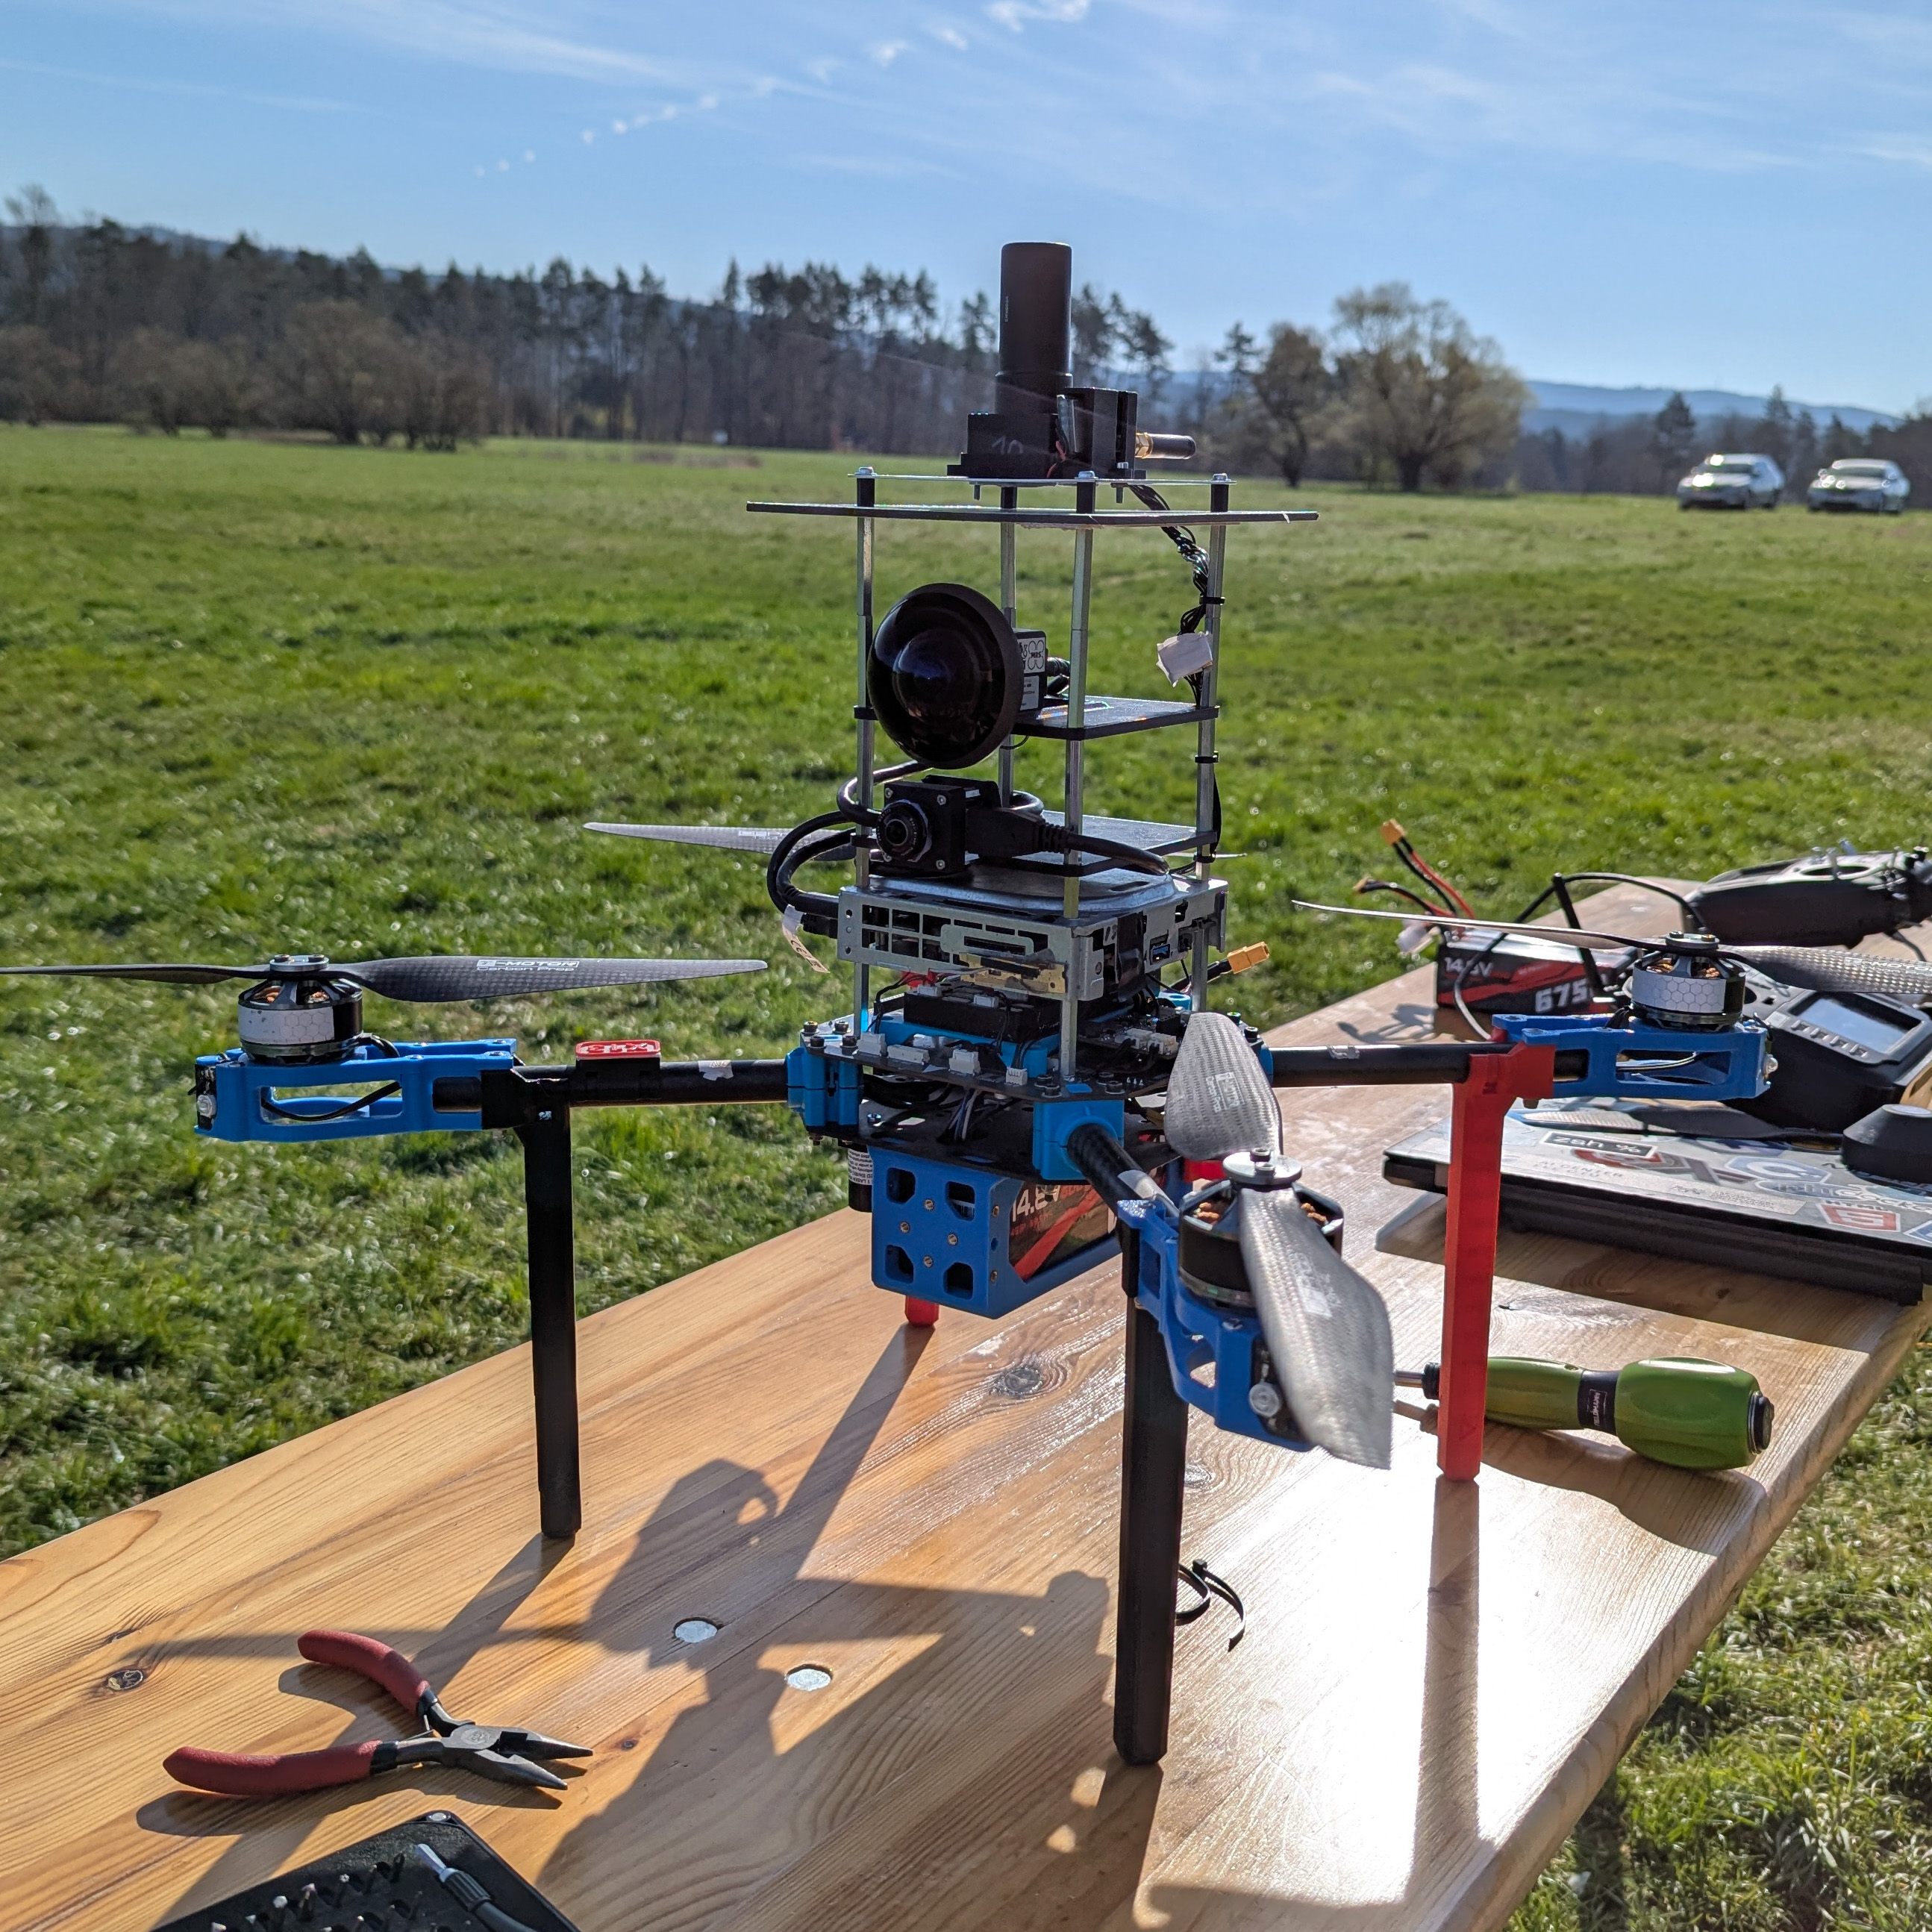
\includegraphics[width=0.60\textwidth]{./fig/photos/uav37.jpg}
            
            \caption{UAV33 and UAV37}
            \label{fig:calib2}
        \end{figure}
    \end{column}
\end{columns}

\end{frame}

% -------------------- QUESTIONS ----------------------

% \begin{frame}[shrink=20]
%     \frametitle{References}
%     %\nocite{*}
%     \begingroup
%     \tiny
%     \printbibliography[heading=none]
%     \endgroup

%     %The source code can be found at:
    
%     %\url{https://github.com/kubakubakuba/mrs-uvdar-distance-estimator}.
% \end{frame}

\section{Otázky}

\questionframe
    {Jaké jsou další metody, které by bylo možné využít k lokalizaci namísto PnP a proč bylo PnP použito namísto jich?}
    {
    \footnotesize{
    Metody pro lokalizaci založené na viditelném světle můžeme rozdělit do následujících kategorií:
        \begin{itemize}
            \item Fingerprinting - odhad polohy na základě předem naměřených referenčních vzdáleností (nutnost nasbírat velký dataset referenčních dat)
            \item Time/Angle of Arrival - je využit rozdíl času/úhlů doražených signálů
            \item Received Signal Strength - metoda často využívá fotodiody k získání poměru síly signálů
            \item Image Sensing - například PnP
        \end{itemize}
    }
    Metoda PnP bylo použita pro její možnost odhadu polohy pomocí výsledného obrazu z eventové kamery, poskytuje silný základ
    pro odhad polohy z relativně malého množství obdržených dat.
    %todo{double check, maybe rewrite}
    }

\questionframe
    {Proč se používá ”fisheye” čočka jako senzor?}
    {
    Kvůli jejímu velkému zornému poli (FOV).
    Čím větší je její FOV, tím spíše jsme schopni detekovat prolétající dronu v našem zorném poli.
    }

\questionframe
    {Z jakého důvodu ve Figure 4.4 dochází k výraznému zvýšení počtu eventů pro 20kHz?}
    {Jedná se o šum kamery, jelikož jsou data pro každou frekvenci normalizována vzhledem k počtu eventů naměrených na jednom metru.
    Při modulační frekvenci 20kHz byly při nastavených parametrech detekovány spíše eventy způsobené šumem,
    než reálné eventy vygenerované jako reakce na změnu jasu LED diod. Velikost obrazu LED diody je porovnatelná s velikostí šumových eventů.
    }
    {
    \vspace{-0.4cm}
    \begin{figure}
        \centering
        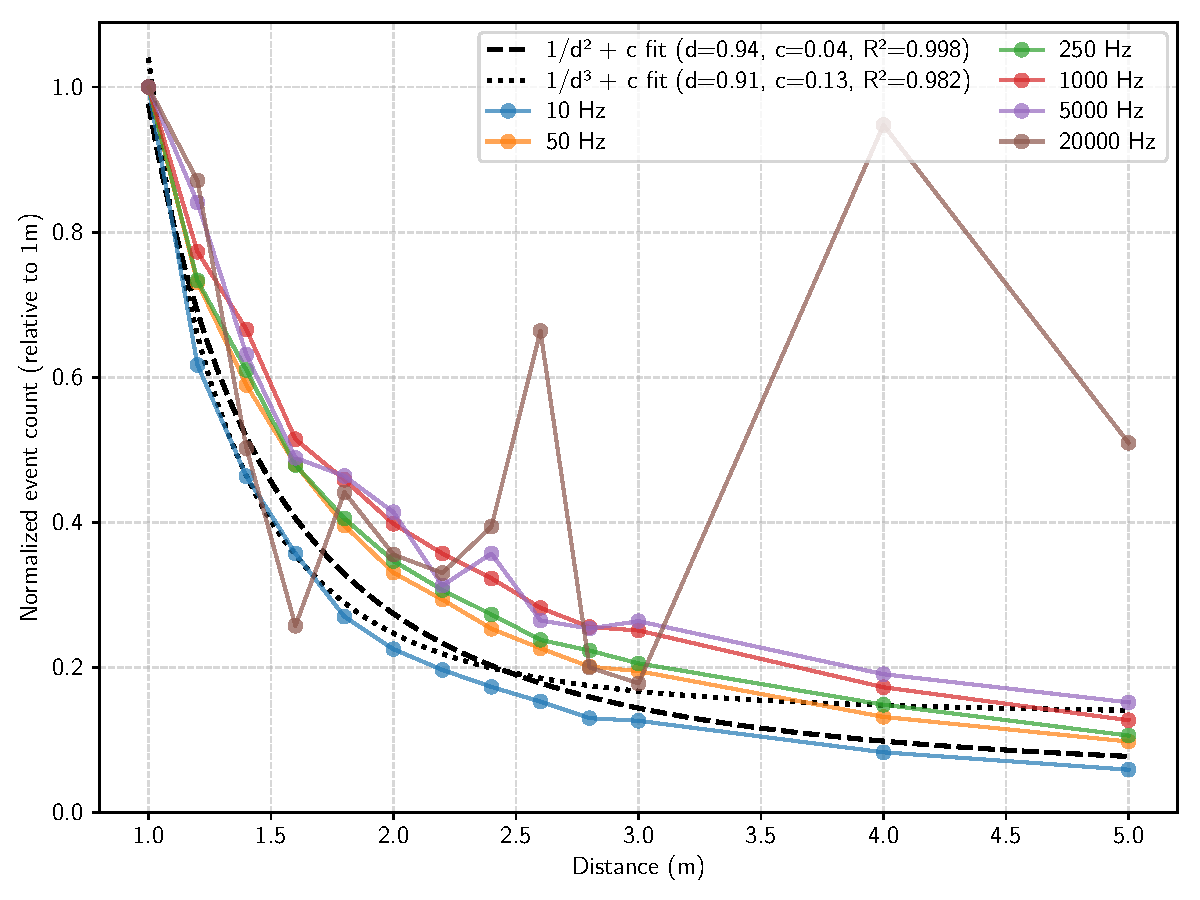
\includegraphics[width=0.45\textwidth]{../fig/pgfplot/build/inv_square.pdf}
        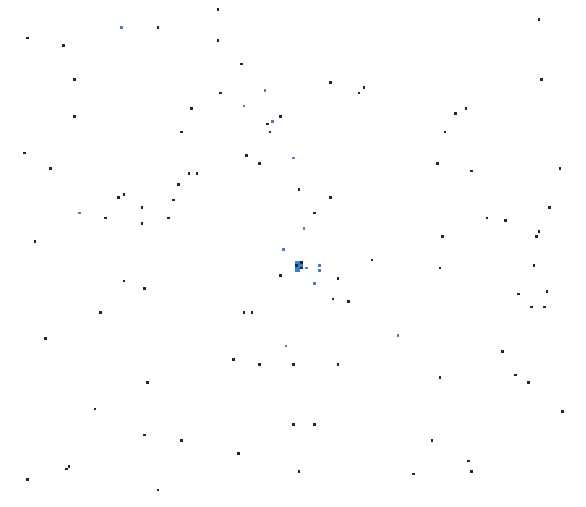
\includegraphics[width=0.40\textwidth]{../fig/photos/event_noise.png}
        \label{fig:fit2}
    \end{figure}
    }

\questionframe
    {Jak si vysvětlujete velkou varianci chyb při kalibraci ”fisheye” čočky? (Kapitola 4.2)}
    {
    Velká variance chyby byla nejspíše způsobena relativní nepřesností při výběru středů detekovaných shluků pixelů napříč kalibračními snímky.
    Nutno podotknout, že chyba se pohybuje pouze v řádu nižších jednotek pixelů ($\sim 1$px).
    
    %\todo{? double check ?}
    }
    {
    \begin{figure}[H]
	\centering
	  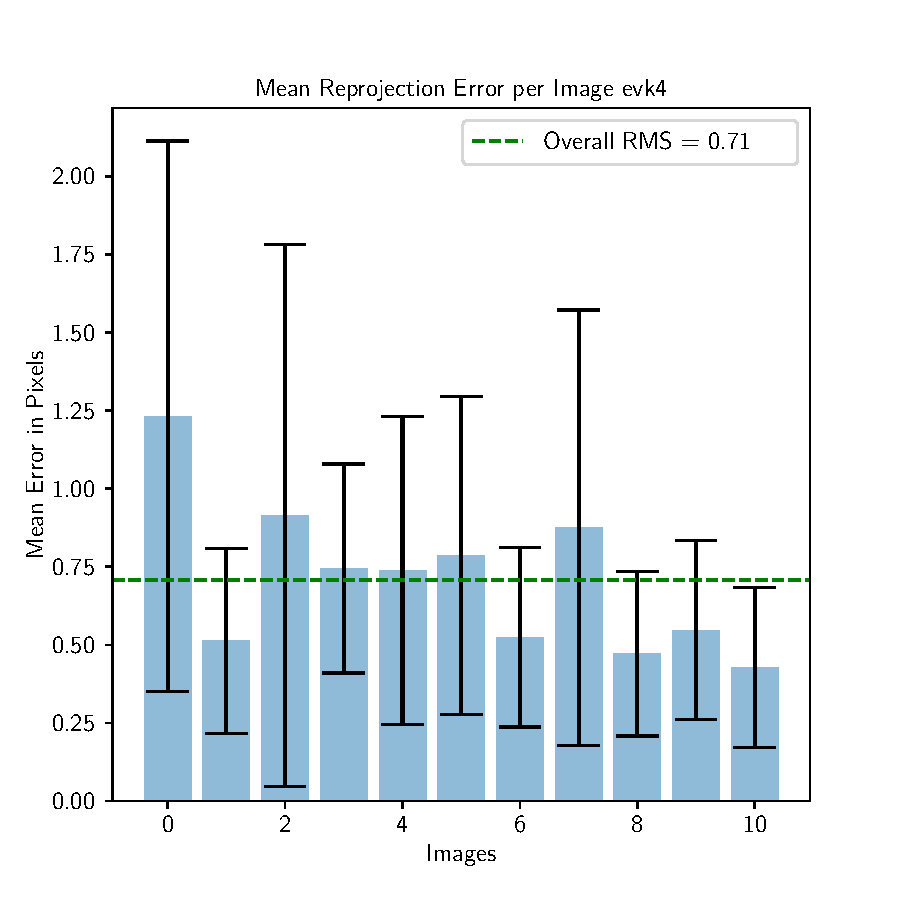
\includegraphics[width=0.42\textwidth]{../fig/pgfplot/build/evk4_reprojection_error_new.pdf}
	  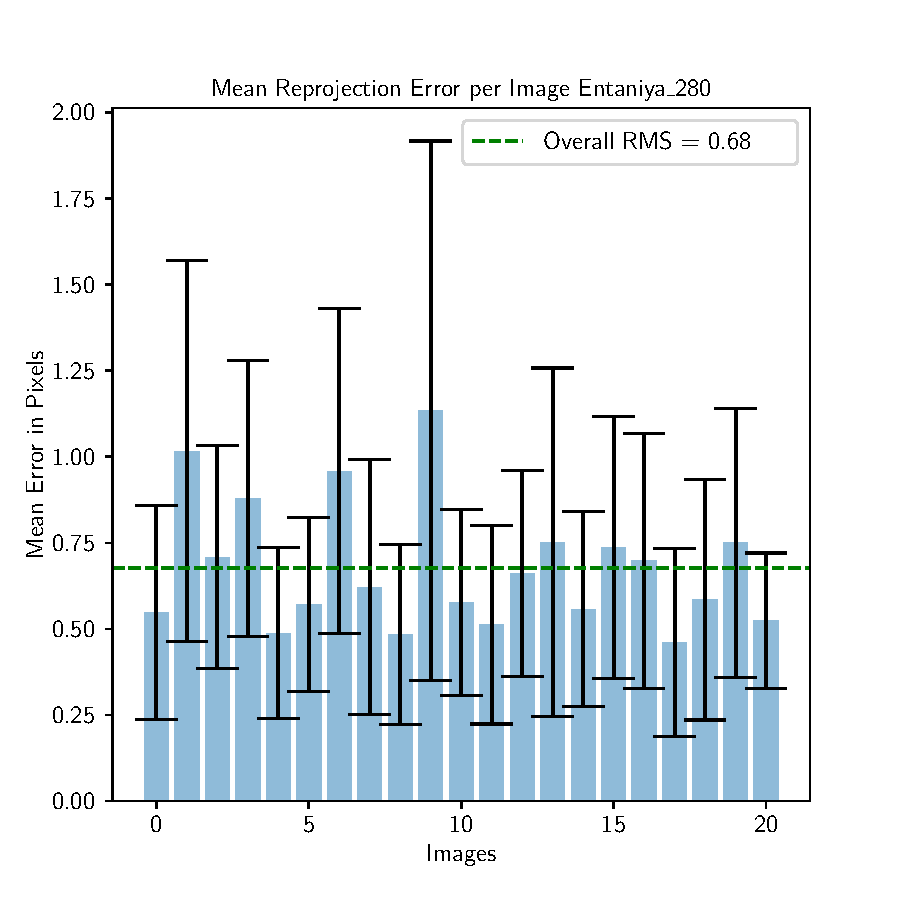
\includegraphics[width=0.42\textwidth]{../fig/pgfplot/build/err_280_new.pdf}
	% \caption{
 %           Pose estimation results, with the estimated pose highlighted in green, and the real pose of the UAVs highlighted in red and blue.
 %        }
	\label{fig:lenserrors}
\end{figure}

	}

\questionframe
    {Je průměrná chyba lokalizace (2.45 metru) vzhledem k měřeným vzdálenostem přijatelná pro praktické použití?}
    {
    Na vzdálenostech testovaných při experimentu s létajícími UAV (15 - 20 metrů) je chyba přijatelná, jelikož má samotná drona dost času reagovat na
    možné přiblížení. Navržený algoritmus navíc odhaduje vzdálenost spíše nižší, než je její reálná hodnota.
    
    Na~nižších vzdálenostech by chyba odhadu měla být řádově nižší, díky přesnější detekci lokace středů LED identifikátorů
    (ověřeno ve statickém experimentu).
    
    %\todo{? double check ?}
    }

\end{document}